\documentclass[12pt, twoside]{article}
\usepackage[utf8]{inputenc}
\usepackage[english,russian]{babel}

\usepackage{amsthm}
\usepackage{a4wide}
\usepackage{graphicx}
\usepackage{caption}
\usepackage{amssymb}
\usepackage{amsmath}
\usepackage{mathrsfs}
\usepackage{euscript}
\usepackage{graphicx}
\usepackage{subfig}
\usepackage{caption}
\usepackage{color}
\usepackage{bm}
\usepackage{tabularx}
\usepackage{adjustbox}


\usepackage[toc,page]{appendix}

\usepackage{comment}
\usepackage{rotating}

\DeclareMathOperator*{\argmax}{arg\,max}
\DeclareMathOperator*{\argmin}{arg\,min}

\newtheorem{theorem}{Теорема}
\newtheorem{lemma}[theorem]{Лемма}
\newtheorem{definition}{Определение}[section]

\numberwithin{equation}{section}

\newcommand*{\No}{No.}
\begin{document}

\title{\bf Анализ свойств локальных моделей в задачах кластеризации квазипериодических временных рядов\thanks{Работа выполнена при поддержке РФФИ и правительства РФ.}}
\date{}
\author{}
\maketitle

\begin{center}
\bf
А.\,В.~Грабовой\footnote{Московский физико-технический институт, grabovoy.av@phystech.edu}, В.\,В.~Стрижов\footnote{Московский физико-технический институт, strijov@ccas.ru}

\end{center}

{\centering\begin{quote}
\textbf{Аннотация:} Данная работа посвящена анализу периодических сигналов во временных рядах с целью распознавания физических действий человека с помощью акселерометра. 
Предлагается метод кластеризации точек временного ряда для поиска характерных квазипериодических сегментов временного ряда. 
Временные ряды являются объектами сложной структуры, для которых не задано исходное признаковое описание. 
%Для построения их признакового описания используется метод главных компонент для локального снижения размерности фазового пространства. 
В качестве признакового описания точек временного ряда рассматриваются главные компоненты локальной окрестности фазовой траектории вблизи данной точки. 
Для оценки близости двух точек временного ряда вычисляется расстояние между данными точками в построенном пространстве признаков. 
При помощи матрицы попарных расстояний между точками временного ряда выполняется кластеризация данных точек. 
Для анализа качества представленного алгоритма проводятся эксперименты на синтетических данных и данных полученных при помощи мобильного акселерометра. 
Проводится эксперимент с поиском начала квазипериодических сегментов внутри каждого кластера.


\smallskip
\textbf{Ключевые слова}: временные ряды; кластеризация; сегментация; распознание физической активности; метод главных компонент.

\smallskip
\textbf{DOI}: 00.00000/00000000000000
\end{quote}
}

\section{Введение}
Анализ физической активности человека производится при помощи мобильных телефонов, разумных часов~\cite{kwapisz2010, wang2014}. 
Эти устройства используют акселерометр, гироскоп и магнитометр. 
Цель данной работы заключается в  разметке и распознавании человеческой активности~\cite{Ignatov2015, Olivares2012, cinar2018}, а также поиска начала каждого действия~\cite{motrenko2015}. 
Примерами одного сегмента действия служит шаг, шаг бега, приседание, прыжок и др. 
Исследуются последовательности, которые состоят не менее чем из двух подряд идущих сегментов, которые соответствуют одному и тому жу типу человеческой активности.

\begin{figure}[h!t]\center
\subfloat[]
{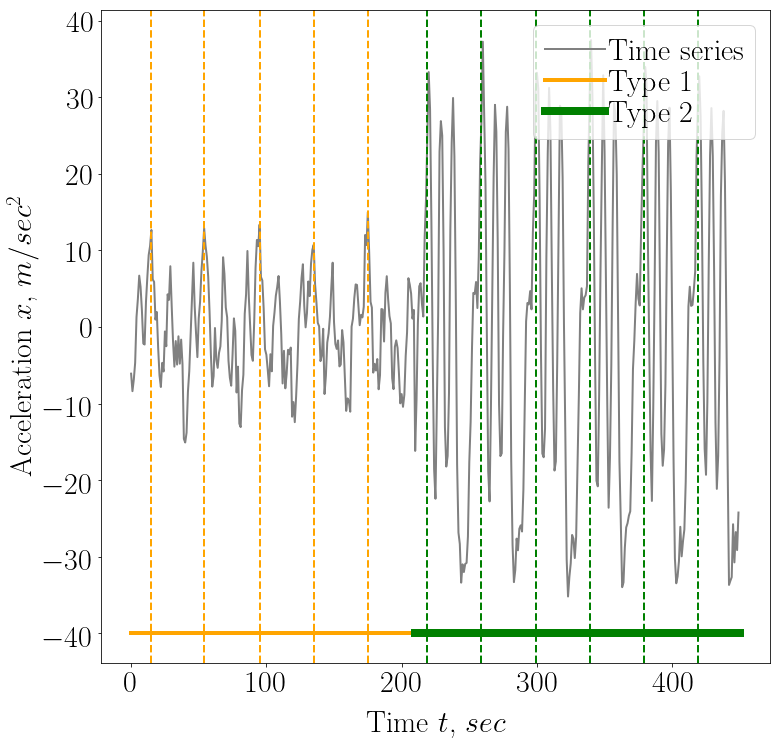
\includegraphics[width=0.5\textwidth]{results/example}\label{example:1}}
\subfloat[]
{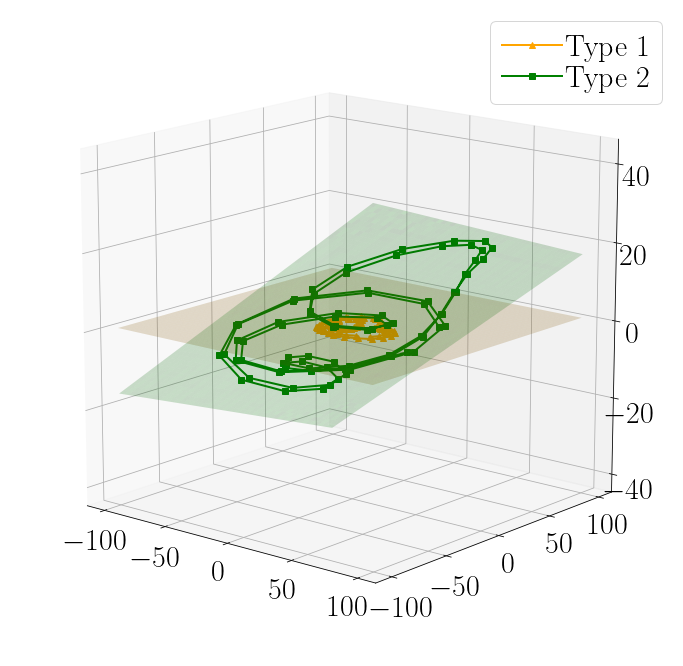
\includegraphics[width=0.5\textwidth]{results/example_phase}\label{example:2}}\\
\caption{Временной ряд, с разметкой на кластеры: a) временной ряд с ассесорской разметкой на кластеры и выделением начала квазипериодического сегмента; b) проекция фазовых траекторий на первые две главные компоненты }
\end{figure}

Временные ряды~---~это объекты сложной структуры. 
При их классификации значимую роль играет модель построения признакового пространства.
Примером метода построения признакового пространства для временного ряда является метод экспертного задания порождающих функций~\cite{kwapisz2010}. 
В~\cite{lukashin2003} рассматривается метод построения признаков на основе гипотезы порождения данных. 
В~\cite{Ivkin2015} рассматривается комбинированное признаковое описание на основе данных методов. 
В~\cite{Katrutsa2015} рассматривается проблема построение признакового пространства и предлагается критерий избыточности выбранных признаков.

В данной работе объектом анализа и кластеризации является точка на оси времени. 
Решается задача кластеризации точек временного ряда. При \textit{кластеризации} каждой точке временного ряда ставится в соответствие метка из конечного множества меток. 
Каждая метка соответствует одному характерному физическому действию. \textit{Сегмент} это часть временного ряда, которая соответствует одному характерному физическому действию, например: шаг, двумя ногами при ходьбе, или шаг, двумя ногами при беге.
Последовательность сегментов, которые соответствуют одному физическому действия образуют \textit{цепочку} действий. 
Предполагается, что цепочка действий образует квазипериодическую последовательность значений временного ряда.
Последовательность точек $\{b_t\}_{t=1}^{N}$ назовем \textit{квазипериодической} с периодом $T$, если для всех $t$ найдется $\Delta$, такое что:
\begin{equation}
\label{eq:int:1}
\begin{aligned}
b_t \approx b_{t+T+\Delta}, \quad \left|\Delta\right| \ll T.
\end{aligned}
\end{equation}
Пример кластеризации и разбиения ряда на сегменты показан на  рис.~\ref{example:1}. Данный ряд разбит на два характерных физических действия, которые обозначаются Type~1 и Type~2. Также данный ряд содержит в себе две квазипериодические цепочки действий.

Решение задачи кластеризации состоит из двух этапов. 
Во-первых, для получения признакового описания временного ряда предлагается алгоритм локальной аппроксимации временного ряда при помощи метода главных компонент~\cite{Shiglavsi1997}. 
Под \textit{локальной} аппроксимацией временного ряда подразумевается, что для признакового описания его точки используется не весь ряд, а только некоторая окрестность данной точки. 
В качестве признакового описания точки временного ряда рассматриваются две главные компоненты \textit{сегмента фазовой траектории} в окрестности данной точки.
На рис.~\ref{example:2} показаны две первые главные компоненты \textit{фазовых тракекторий}, а также проекция фазовых траекторий на эти компоненты.
Они соответствуют разным физическим действиям, которые обозначаются Type~1 и Type~2, внутри одного временного ряда.
Как видно плоскости, которые порождены данными главными компонентами не совпадают. 
Это говорит о том, что наблюдаются различные действия. 
Во-вторых, вводится функция расстояния в построенном пространстве признакового описания. 
Данная функция является расстояниям между двумя подпространствами внутри всего фазового пространства временного ряда.
На рис.~\ref{example:2} данная функция является некоторым расстояниям между двумя плоскостями.
Получив расстояния между точками временного ряда, выполним кластеризацию данных точек.
Задача сегментации внутри каждого кластера решается при помощи метода, который рассмотрен в~\cite{motrenko2015}.

Для решения задачи кластеризации точек временного ряда вводятся предположения. 
Предполагается, что периоды различных сегментов различаются незначительно, причем известны минимальный и максимальный периоды сегмента и число различных сегментов внутри временного ряда. 
Также предполагается, что тип активности во времени не меняется часто, а также что фазовые траектории разных сегментов являются различными. 

Проверка и анализ метода кластеризации проводится на синтетической и реальной выборках. 
Синтетическая выборка построенная при помощи суммы нескольких первых членов ряда Фурье со случайными коэффициентами. 
Эксперимент по сегментации временного ряда проводился на простых синусоидальных сигналах с произвольной амплитудой и частотой. 
Реальные данные получены при помощи мобильного акселерометра, который снимал показания во время некоторой физической активности человека. 

\section{Анализ литературы}
В~\cite{kwapisz2010} рассматриавется метод построения признакового описания на основе экспертно заданых порождающих функций.
В~\cite{lukashin2003} рассматривается метод построения признаков на основе гипотезы порождения данных. 
В~\cite{Ivkin2015} рассматривается комбинированное признаковое описание на основе данных методов. 
В~\cite{Katrutsa2015} рассматривается проблема построение признакового пространства и предлагается критерий избыточности выбранных признаков.

Работа~\cite{motrenko2015} является ближайшей работой по данной теме. Она заключается в поиске начала сегмента внутри квазипериодического сигнала, который состоит, только из одной цепочки действий. Этот метод основан на исследовании фазового пространства, а именно поиска устойчивой гиперплоскости, которая делит фазовое пространство на две равные части. В качестве начала сегмента выбираются точки, которые находятся близко к данной гиперплоскости. В~\cite{motrenko2015} предлагается выполнить проекцию фазового пространства на первые две главное компоненты, после чего провести устойчивую прямую, выделив начала каждого сегмента. 
Данный метод имеет недостаток в том, что позволяет находить начало только для временного ряда, который состоит из квазипериодического сигнала единственного типа.


Также близкой является работа~\cite{cinar2018}.  Данная работа заключается в поиске периодической структуры внутри ряда при помощи модели LSTM с модифицированным механизмом Attention. Предполагается, что механизм Attention будет давать максимальное значение score в точках, которые удаленны от данной на целое количество периодов.

\section{Постановка задачи кластеризации точек временного ряда}

Задан временной ряд
\begin{equation}
\label{eq:st:1}
\begin{aligned}
\textbf{x} \in \mathbb{R}^{N},
\end{aligned}
\end{equation}
где~$N$ число точек временного ряда. Он состоит из последовательности сегментов:
\begin{equation}
\label{eq:st:2}
\begin{aligned}
\textbf{x} = [\textbf{v}_1, \textbf{v}_2, \cdots, \textbf{v}_M],
\end{aligned}
\end{equation}
где~$\textbf{v}_i$ некоторый сегмент из множества сегментов~$\mathbf{V}$, которые встречаются в данном ряде. 
Причем для всех~$i$ либо~$[\textbf{v}_{i-1},\textbf{v}_{i}]$ либо~$[\textbf{v}_{i},\textbf{v}_{i+1}]$  является цепочкой действий. Пусть множество~$\mathbf{V}$ удовлетворяет следующим свойствам:

\begin{equation}
\label{eq:st:3}
\begin{aligned}
\left|\mathbf{V}\right| = K, \quad \textbf{v} \in \mathbf{V}~\left|\textbf{v}\right| \leq T,
\end{aligned}
\end{equation}
где~$\left|\mathbf{V}\right|$ число различных действий в множестве сегментов $\mathbf{V},$~$\left|\textbf{v}\right|$ длина сегмента, а~$K$ и~$T$ это число различных действий во временном ряде и длина максимального сегмента соответсвенно.

Рассматривается отображение
\begin{equation}
\label{eq:st:4}
\begin{aligned}
a : t \to \mathbb{Y} = \{1,\cdots, K\}, 
\end{aligned}
\end{equation}
где~$t \in \{1,\cdots, N\}$ некоторый момент времени, на котором задан временной ряд.
Требуется, чтобы отображение~$a$ удовлетворяло следующим свойствам:

\begin{equation}
\label{eq:st:5}
\begin{aligned}
\begin{cases}
    a\left(t_1\right) = a\left(t_2\right), &  \text{если в моменты } t_1, t_2 \text{ совершается один тип действий}\\
    a\left(t_1\right) \not= a\left(t_2\right), &  \text{если в моменты } t_1, t_2 \text{ совершаются разные типы действий }
\end{cases}
\end{aligned}
\end{equation}

Пусть задана некоторая асессорская разметка временного ряда:
\begin{equation}
\label{eq:st:6}
\begin{aligned}
\textbf{y} \in \{1,\cdots,K\}^{N}.
\end{aligned}
\end{equation}
Тогда ошибка алгоритма~$a$ на временном ряде~$\textbf{x}$ представляется в следующем виде:
\begin{equation}
\label{eq:st:7}
\begin{aligned}
S = \frac{1}{N}\sum_{t=1}^{N}[y_t = a\left(t\right)],
\end{aligned}
\end{equation}
где~$t$~---~момент времени,~$y_t$ асессорская разметка~$t$-го момента времени для заданого временного ряда.

\section{Кластеризация точек}
Рассмотрим фазовую траекторию временного ряда~$\textbf{x}$:
\begin{equation}
\label{eq:cl:1}
\begin{aligned}
\mathbf{H} = \{\textbf{h}_t| \textbf{h}_t = [x_{t-T}, x_{t-T+1}, \cdots, x_{t}],~T\leq t\leq N\},
\end{aligned}
\end{equation}
где $\textbf{h}_t$~---~точка фазовой траектории.

Информация об длине максимального сегмента~$T$ внутри временного ряда позволяет разбить фазовую траекторию на сегменты из~$2T$ векторов:
\begin{equation}
\label{eq:cl:2}
\begin{aligned}
\mathbf{S} = \{\textbf{s}_t| \textbf{s}_t = [\textbf{h}_{t-T}, \textbf{h}_{t-T+1}, \cdots, \textbf{h}_{t+T-1}],~T\leq t\leq N-T\},
\end{aligned}
\end{equation}
где $\textbf{s}_t$~---~это сегмент фазовой траектории. Данные сегменты имеют всю локальную информацию об временном ряде, так как содержит всю информацию на периоде до момента времени~$t$ и информацию о периоде после момента времени~$t$.

В качестве признакового описания точки временного ряда $t$ рассматриваются главные компоненты~$\textbf{W}_t$ для~$T\text{-мерных}$ сегментов~$\textbf{s}_t$. Сегмент~$\textbf{s}_t$ проекцируется на подпространство размерности два при помощи метода главных  компонент~$\textbf{z}_t~=~\textbf{W}_t\textbf{s}_t$. Получаем:

%Каждое~$T\text{-мерное}$ подпространство~$\textbf{s}_t$ проектируется на подпространство значительно меньшей размерности при помощи метода главных  компонент~$\textbf{z}_t~=~\textbf{W}_t\textbf{s}_t$. Получим представление базисных векторов~$\textbf{W}_t$, а также собственные числа, которые соответствуют данным базисным векторам каждого подпространства~$\textbf{s}_t$ в~$T\text{-мерном}$ пространстве:
\begin{equation}
\label{eq:cl:3}
\begin{aligned}
\mathbf{W} = \{\textbf{W}_t| \textbf{W}_t = [\lambda^1_t\textbf{w}^1_t, \lambda^2_t\textbf{w}^2_t]\}, \quad \bm{\Lambda} = \{\bm{\lambda}_t| \bm{\lambda}_t=[\lambda^1_t, \lambda^2_t]\},
\end{aligned}
\end{equation}
где~$[\textbf{w}^1_t, \textbf{w}^2_t]$ и~$[\lambda^1_t, \lambda^2_t]$ это базисные векторы и соответствующие им собственные для сегмента фазовой траектории~$\textbf{s}_t$.

Для кластеризации точек временного ряда рассмотрим функцию расстояния между элементами~$\mathbf{W}_{t_1},\mathbf{W}_{t_2}$:
\begin{equation}
\label{eq:cl:4}
\begin{aligned}
\rho\left(\textbf{W}_1, \textbf{W}_2\right) = \max\left(\max_{\textbf{e}_2 \in \textbf{W}_2} d_{1}\left(\textbf{e}_2\right), \max_{\textbf{e}_1 \in \textbf{W}_1} d_{2}\left(\textbf{e}_1\right)\right),
\end{aligned}
\end{equation}
где ~$\textbf{e}_i$ это базисный вектор пространства~$\textbf{W}_i,$ а~$d_i\left(\textbf{e}\right)$ является расстоянием от вектора~$\textbf{e}$ до пространства~$\textbf{W}_i$.

\begin{comment}
\begin{theorem}
Пусть задано множество подпространств~$\mathbb{W}$ пространства~$\mathbb{R}^{n}$. Каждое подпространство которого задается базисом~$\mathbf{W}_i\in \mathbf{W}$, тогда функция расстояния~$\rho\left(\textbf{W}_1, \textbf{W}_2\right)$ является метрикой заданой на множестве базисов~$\mathbf{W}$:
\begin{equation}
\begin{aligned}
\rho\left(\textbf{W}_1, \textbf{W}_2\right) = \max\left(\max_{\textbf{e}_2 \in \textbf{W}_2} d_{1}\left(\textbf{e}_2\right), \max_{\textbf{e}_1 \in \textbf{W}_1} d_{2}\left(\textbf{e}_1\right)\right),
\end{aligned}
\end{equation}
где~$\textbf{e}_i$ это базисный вектор из~$\textbf{W}_i$, a~$d_i\left(\textbf{e}\right)$ является расстоянием от вектора~$\textbf{e}$ до пространства заданого базисом~$\textbf{W}_i$.
\end{theorem}

В силу теоремы~\ref{th:1} функция расстояния~(\ref{eq:cl:4}) является метрикой, доказательство данной теоремы представлено в приложении \ref{ProofTheorem1}. 
\end{comment}

В случае, когда все подпространства~$\textbf{W}_t$ имеют размерность два, расстояние~$\rho\left(\textbf{W}_1, \textbf{W}_2\right)$ имеет следующую интерпретацию:

\begin{equation}
\label{eq:cl:5}
\begin{aligned}
\rho\left(\textbf{W}_1, \textbf{W}_2\right) = \max_{\{\textbf{a},\textbf{b},\textbf{c}\} \subset \textbf{W}_1\cup \textbf{W}_2 } V\left(\textbf{a},\textbf{b},\textbf{c}\right), 
\end{aligned}
\end{equation}
где~$\textbf{W}_1\cup\textbf{W}_2$ это объединение базисных векторов первого и второго пространства,~$V\left(\textbf{a},\textbf{b},\textbf{c}\right)$~---~объем параллелепипеда построенного на векторах~$\textbf{a}, \textbf{b}, \textbf{c}$, которые являются столбцами матрицы~$\textbf{W}_1\cup\textbf{W}_2$.


Рассмотрим расстояние между собственными числами:
\begin{equation}
\label{eq:cl:6}
\begin{aligned}
\rho\left(\bm{\lambda}_1, \bm{\lambda}_2\right) = \sqrt[]{\left(\bm{\lambda}_1 - \bm{\lambda}_2\right)^{\mathsf{T}}\left(\bm{\lambda}_1 - \bm{\lambda}_2\right)}.
\end{aligned}
\end{equation}
%Функция расстояния~$\rho\left(\bm{\lambda}_1, \bm{\lambda}_2\right)$ является метрикой в пространстве~$\mathbb{R}^2$.
%Матрица попарных расстояний между базисными векторами~$\textbf{M}_{\text{c}}$ и матрица попарных расстояний между собственными значениями~$\textbf{M}_{\text{l}}$ для временного ряда~$\textbf{x}$:
%\begin{equation}
%\label{eq:cl:8}
%\begin{aligned}
%\textbf{M}_{\text{c}} = [0, 1]^{N\times N}, \quad \textbf{M}_{\text{l}} = [0, 1]^{N\times N}.
%\end{aligned}
%\end{equation}
Используя выражения~(\ref{eq:cl:5}-\ref{eq:cl:6}) введем расстояние между двумя точками~$t_1, t_2$ временного ряда, а также рассмотрим матрицу попарных расстояний~$\textbf{M}$ между точками данного ряда:
\begin{equation}
\label{eq:cl:9}
\begin{aligned}
\rho\left(t_1, t_2\right) = \rho\left(\textbf{W}_1, \textbf{W}_2\right) + \rho\left(\bm{\lambda}_1, \bm{\lambda}_2\right), \quad \textbf{M} =  \mathbb{R}^{N\times N},
\end{aligned}
\end{equation}
где %~$\rho\left(t_1, t_2\right)$ является метрикой, так как является суммой двух метрик,
матрица~$\textbf{M}$ является матрицей попарных расстояний между всеми парами точек~$t$ временного ряда~$\textbf{x}$.
Используя матрицу попарных расстояний~$\textbf{M}$ выполним кластеризацию моментов времени~$t$ временного ряда~\eqref{eq:st:4}:

%\begin{equation}
%\label{eq:cl:10}
%\begin{aligned}
%a : t \to \{1,\cdots, K\}, 
%\end{aligned}
%\end{equation}
%где~$t$ некоторый момент времени временного ряда~$\textbf{x}$.


\section{Вычислительный эксперимент}
\subsection{Кластеризация точек временного ряда}
Для анализа свойств предложенного алгоритма кластериизации был проведен вычислительный эксперимент в котором кластеризация точек временного ряда проводилась используя матрицы попарных расстояний ~$(\ref{eq:cl:9})$.

В качестве данных использовались две выборки временных рядов, которые описаны в таблице~\ref{table_1}. 
Выборка Physical Motion это реальные временные ряды полученные при помощи мобильного акселерометра. 
Синтетические временные ряды были построены при помощи нескольких первых слагаемых ряда Фурье со случайными коэффициентами из стандартного нормального распределения. 
Генерация данных состояла из двух этапов. 
На первом этапе генерировались короткие сегменты~$\textbf{v}$ для построения множества~$\mathbf{V}$. 
Вторым этапом генерации выборки~$\textbf{x}$ является следующим случайным процессом:
\begin{equation}
\label{eq:exp:1}
\begin{aligned}
\textbf{x} = [\textbf{v}_{1}, \textbf{v}_{2}, \cdots, \textbf{v}_{M}] + \bm{\varepsilon}, \quad \begin{cases}
    \textbf{v}_{1} \sim \mathcal{U}\left(\mathbf{V}\right),\\
    \textbf{v}_{i} = \textbf{v}_{i - 1}, & \text{с вероятностью}~\frac{3}{4}\\
    \textbf{v}_{i} \sim \mathcal{U}\left(\mathbf{V}\right), & \text{с вероятностью}~\frac{1}{4}
\end{cases},
\end{aligned}
\end{equation}
где~$\mathcal{U}\left(\mathbf{V}\right)$~---~равномерное распределение на объектах из~$\mathbf{V},$ а $\bm{\varepsilon}$ является шумом из нормального распределения.

\begin{table}[h!t]
\begin{center}
\caption{Описание временных рядов в эксперименте кластеризации точек временного ряда}
\label{table_1}
\begin{tabular}{|c|c|c|c|}
\hline
	Ряд,~$\textbf{x}$ &Длина ряда,~$N$& Число сегментов,~$K$&Длина сегмента,~$T$\\
	\hline
	\multicolumn{1}{|l|}{Physical~Motion~1}
	& 900& 2& 40\\
	\hline
	\multicolumn{1}{|l|}{Physical~Motion~2}
	& 900& 2& 40\\
	\hline
	\multicolumn{1}{|l|}{Synthetic~1}
	& 2000& 2& 20\\
	\hline
	\multicolumn{1}{|l|}{Synthetic~2}
	& 2000& 3& 20\\
\hline

\end{tabular}
\end{center}
\end{table}

\begin{figure}[h!t]\center
\subfloat[]
{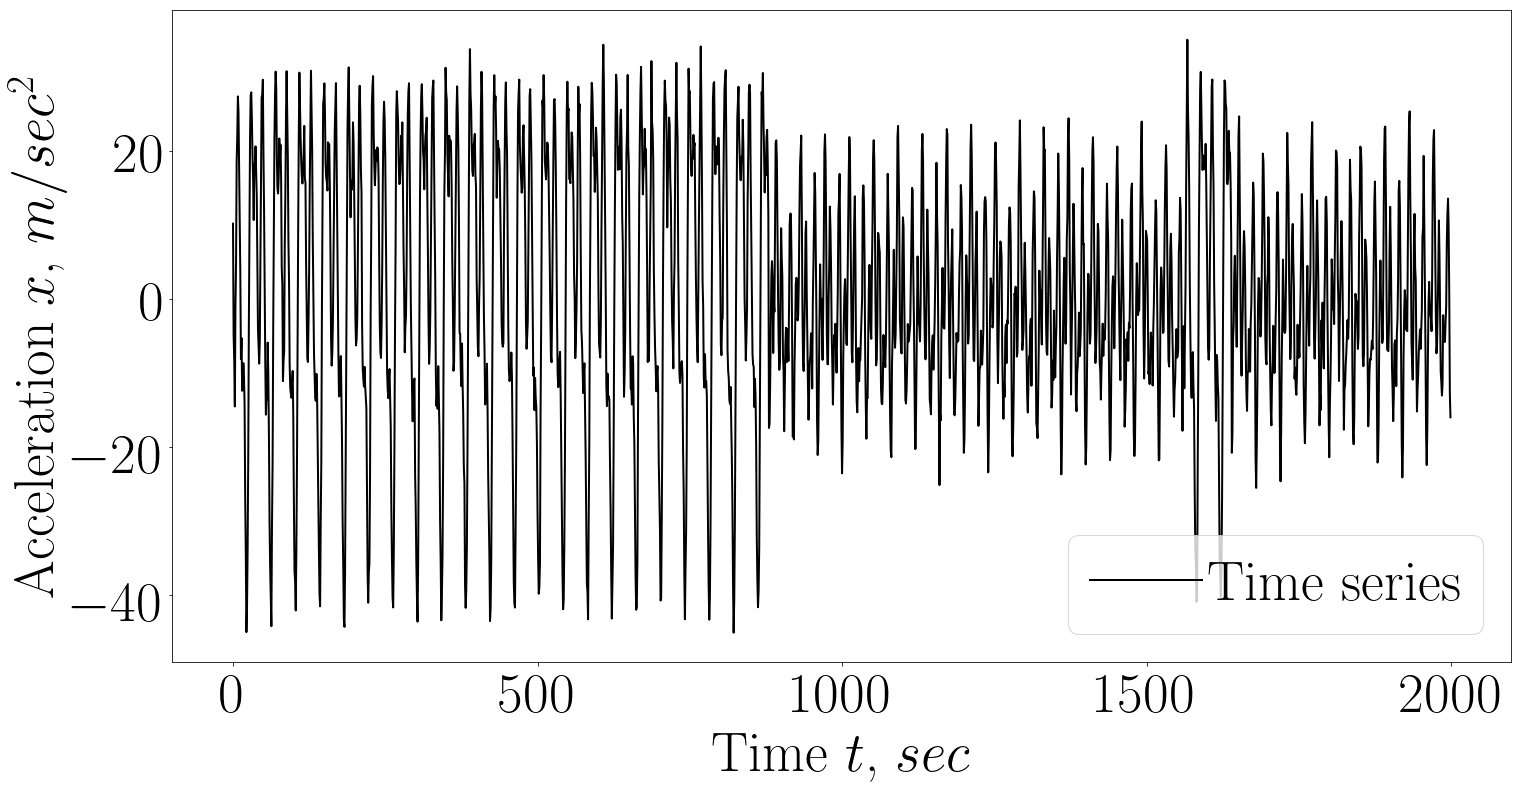
\includegraphics[width=0.5\textwidth]{results/2_patern_2_series}\label{fig_synthetic_series_2}}
\subfloat[]
{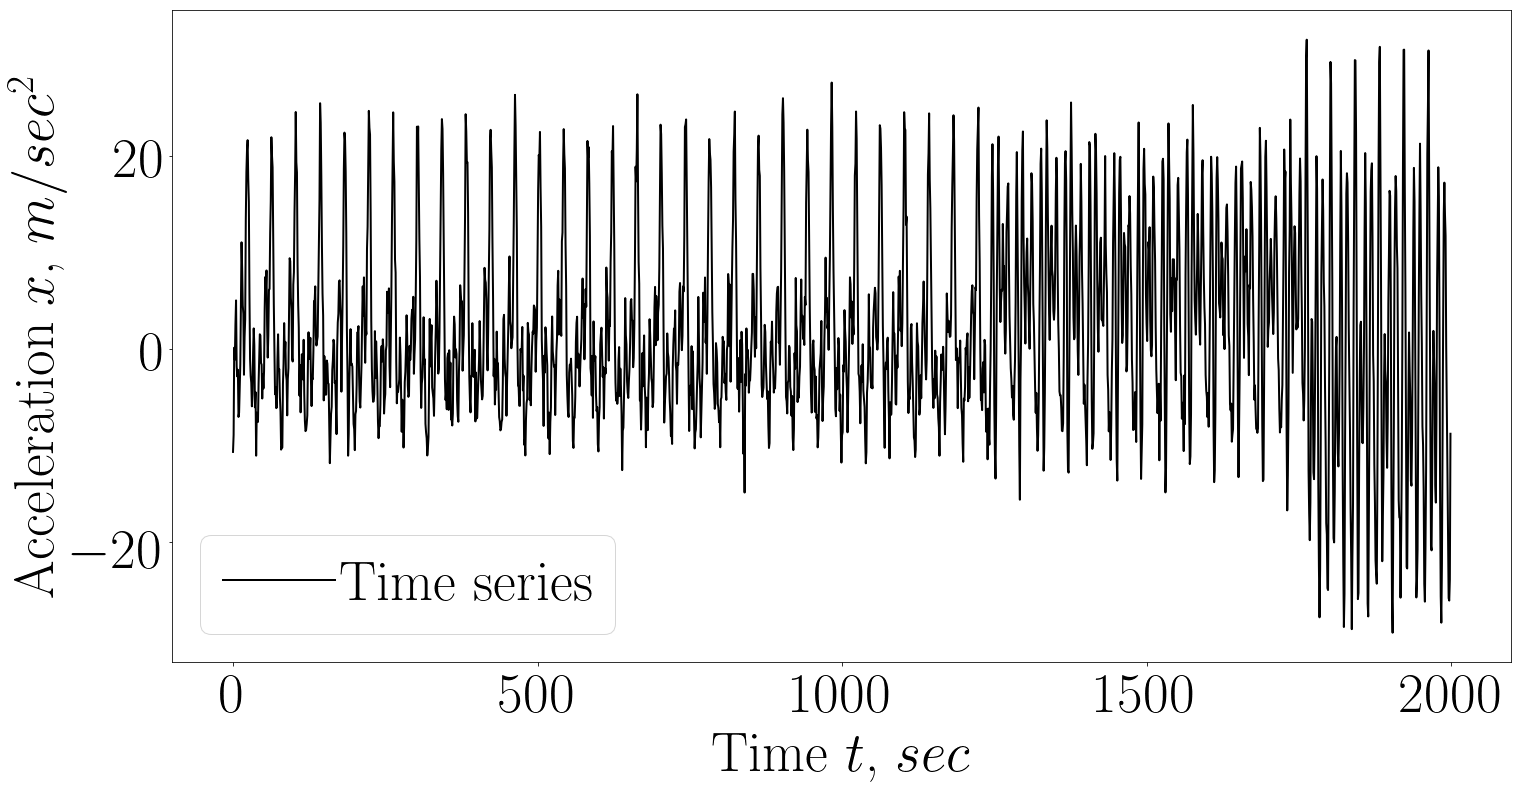
\includegraphics[width=0.5\textwidth]{results/3_patern_2_series}\label{fig_synthetic_series_3}}\\
\caption{Пример синтетически построенных временных рядов: a) для временного ряда Synthetic~1; b) для временного ряда Synthetic~2}
\label{fig_synthetic_series}
\end{figure}

\begin{figure}[h!t]\center
\subfloat[]
{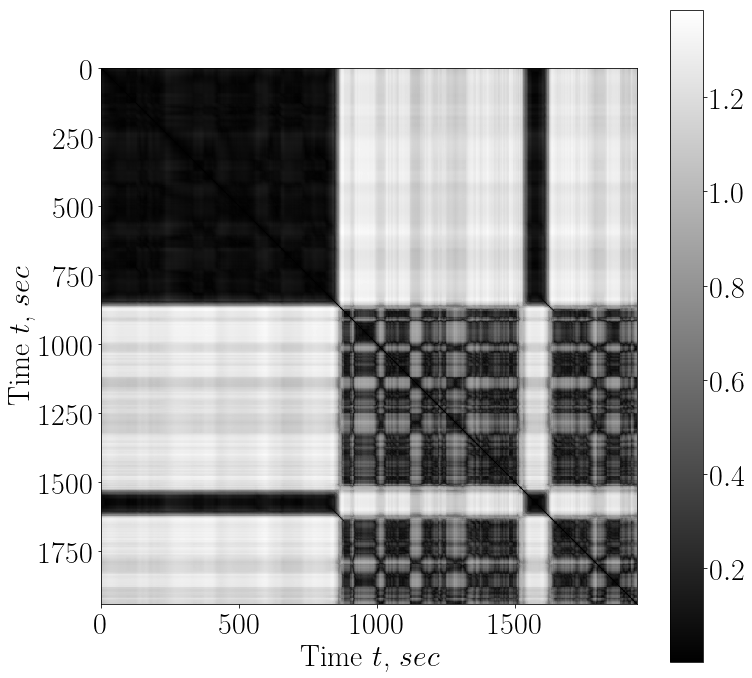
\includegraphics[width=0.5\textwidth]{results/2_patern_2_full}}
\subfloat[]
{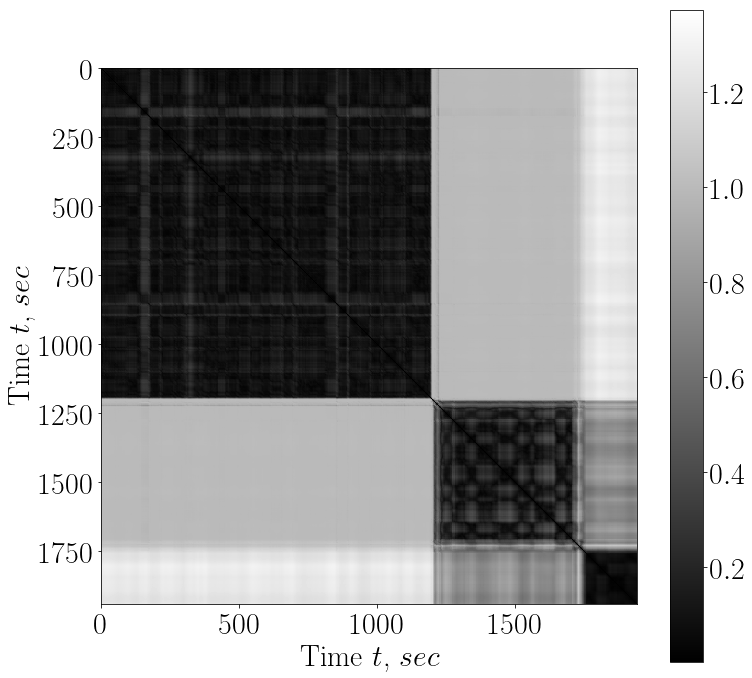
\includegraphics[width=0.5\textwidth]{results/3_patern_2_full}}\\
\caption{Матрица попарных расстояний~$\textbf{M}$ между точками временного ряда: a) для временного ряда Synthetic~1; b) для временного ряда Synthetic~2}
\label{fig_synthetic_distance}
\end{figure}

\begin{figure}[h!t]\center
\subfloat[]
{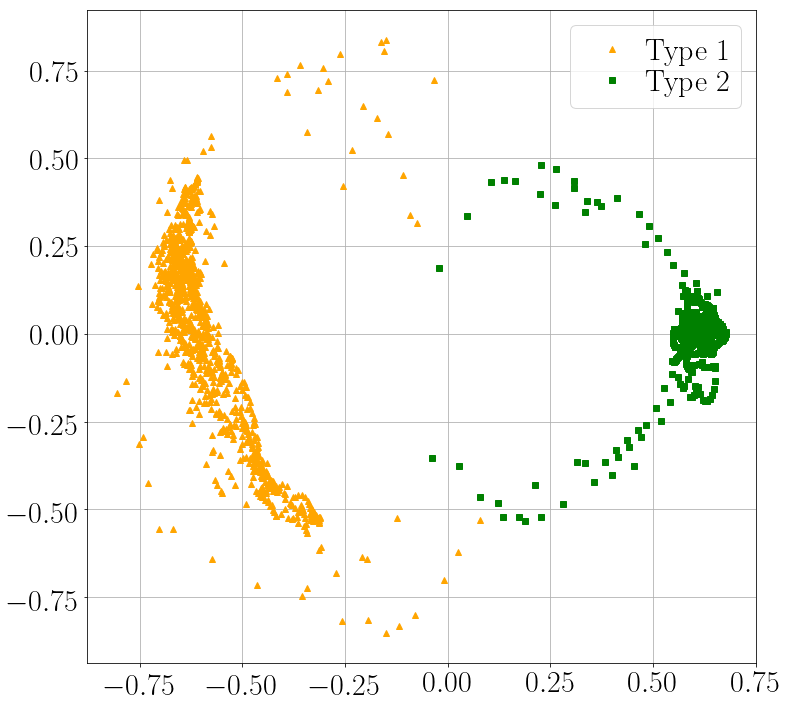
\includegraphics[width=0.5\textwidth]{results/2_patern_2_2D_vector}}
\subfloat[]
{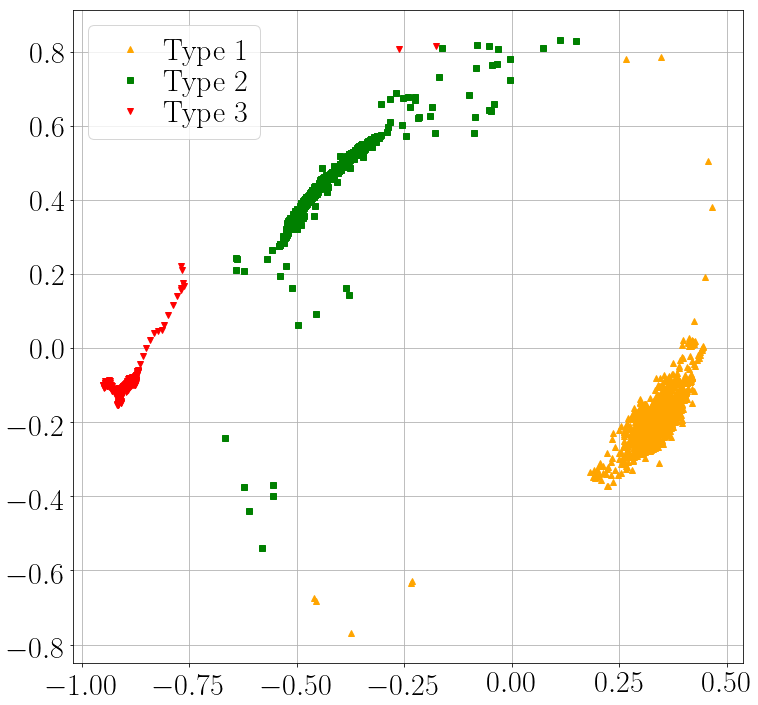
\includegraphics[width=0.5\textwidth]{results/3_patern_2_2D_vector}}\\
\caption{Проекция точек временного ряда на плоскость при помощи матрицы попарных расстояний~$\textbf{M}$: a) для временного ряда Synthetic~1; b) для временного ряда Synthetic~2}
\label{fig_synthetic_2D}
\end{figure}

\begin{figure}[h!t]\center
\subfloat[]
{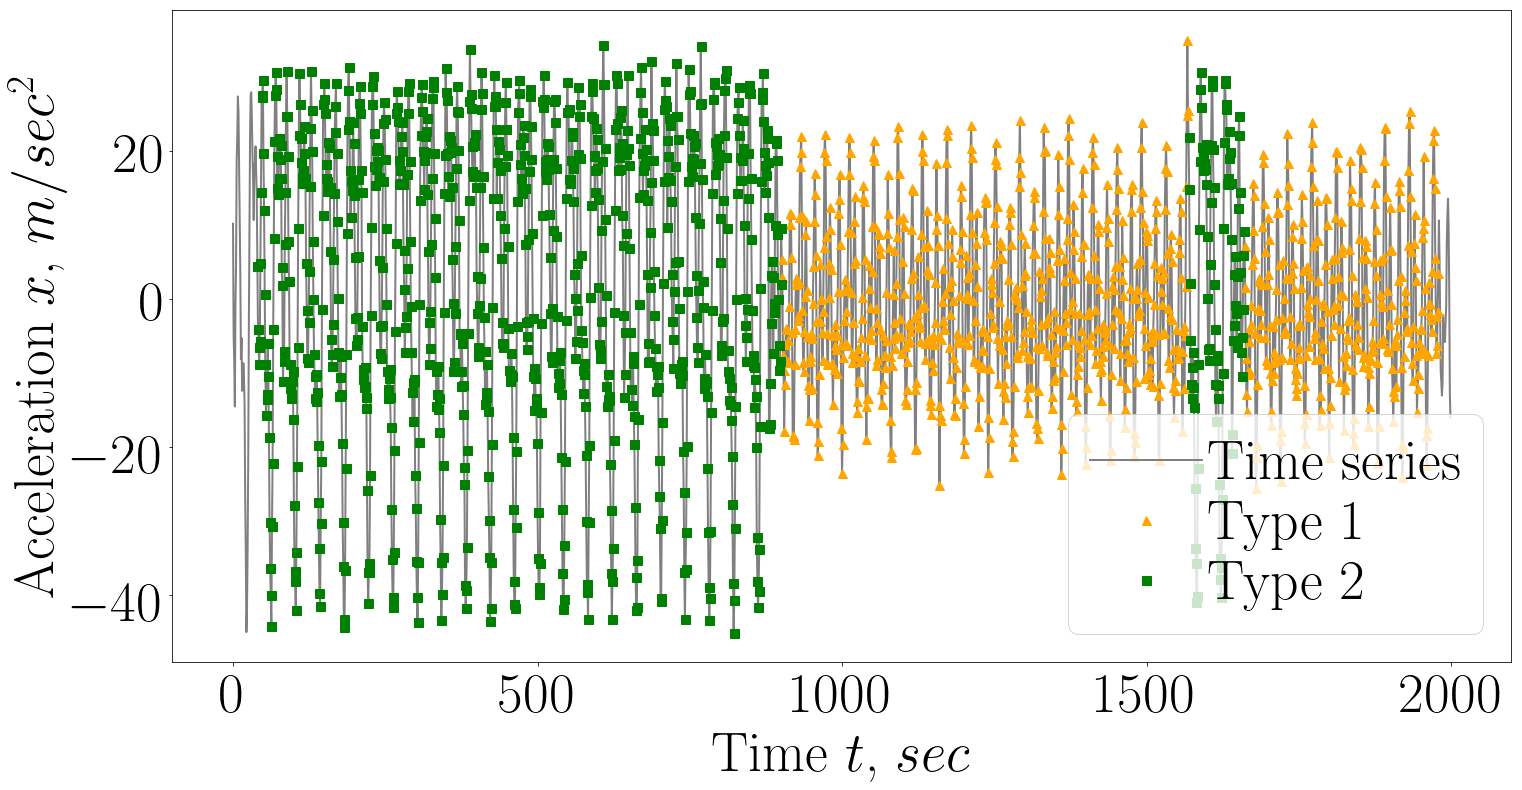
\includegraphics[width=0.5\textwidth]{results/2_patern_2_claster_vector}}
\subfloat[]
{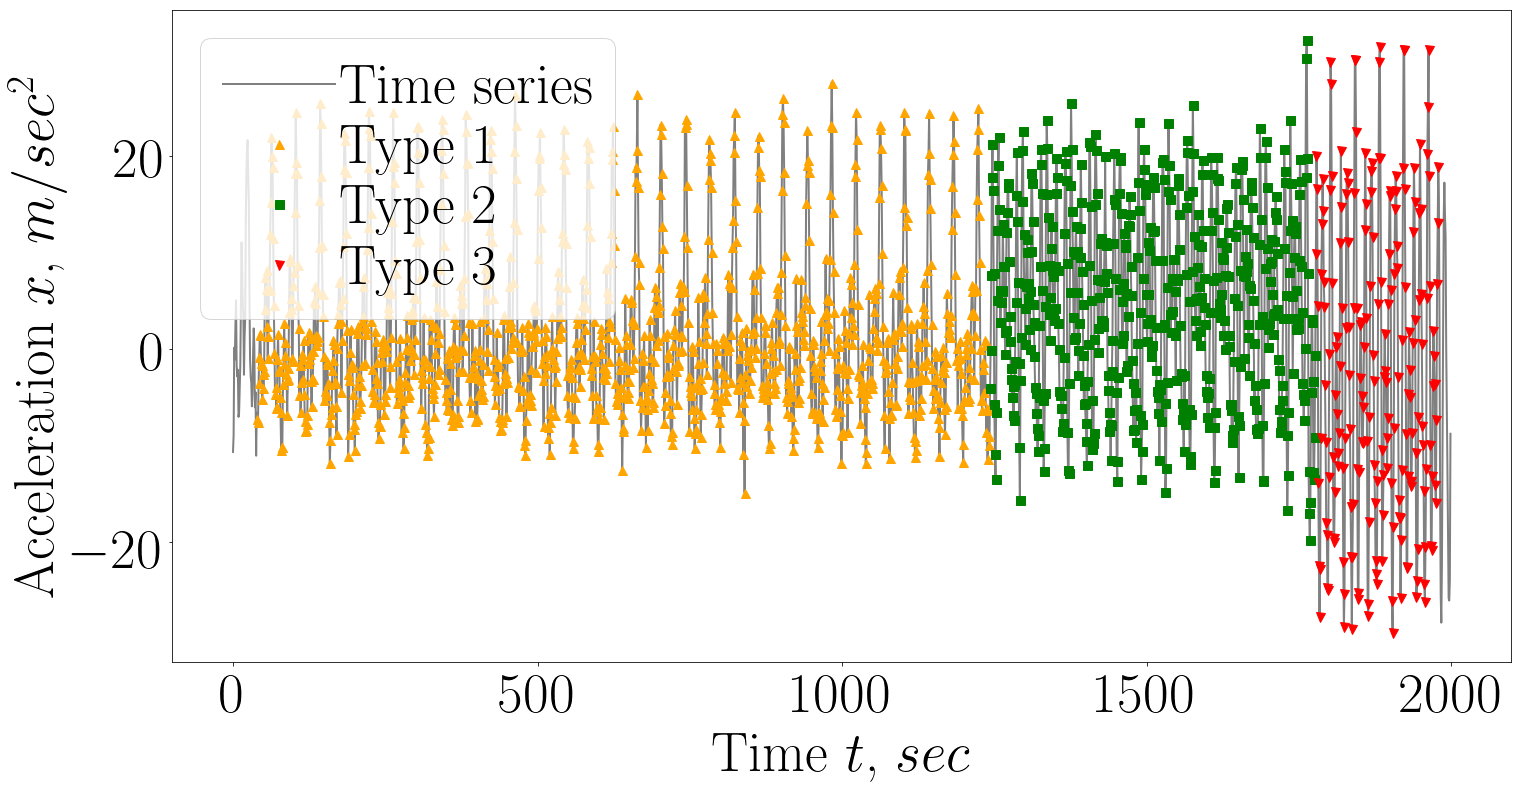
\includegraphics[width=0.5\textwidth]{results/3_patern_2_claster_vector}}\\
\caption{Кластеризация точек временного ряда: a) для временного ряда Synthetic~1; b) для временного ряда Synthetic~2}
\label{fig_synthetic_claster}
\end{figure}


\paragraph{Синтетические данные.}


На рис.~\ref{fig_synthetic_series} приведен пример синтетических временных рядов. 
На рис.~\ref{fig_synthetic_series_2} показан пример ряда в котором число различных сегментов~$K = 2$, а длина каждого сегмента~$T = 20$. 
На рис.~\ref{fig_synthetic_series_3} показан пример ряда в котором число различных сегментов~$K = 3$, а длина каждого сегмента~$T = 20$. 

Рис.~\ref{fig_synthetic_distance} иллюстрирует матрицы попарных расстояний~$\textbf{M}$ между всеми парами точек~$t$ временного ряда, которые построены при помощи~(\ref{eq:cl:9}). 
Используя матрицу попарных расстояний и метод Multidimensional Scaling~\cite{Borg2005} визуализируем точки временного ряда на плоскости. 
На рис.~\ref{fig_synthetic_2D} показана визуализация точек на плоскости и выполнена их кластеризация при помощи метода иерархической кластеризации. 
Иллюстрация кластеров точек временного ряда продемонстрирована на рис.~\ref{fig_synthetic_claster}.

\begin{figure}[h!t]\center
\subfloat[]
{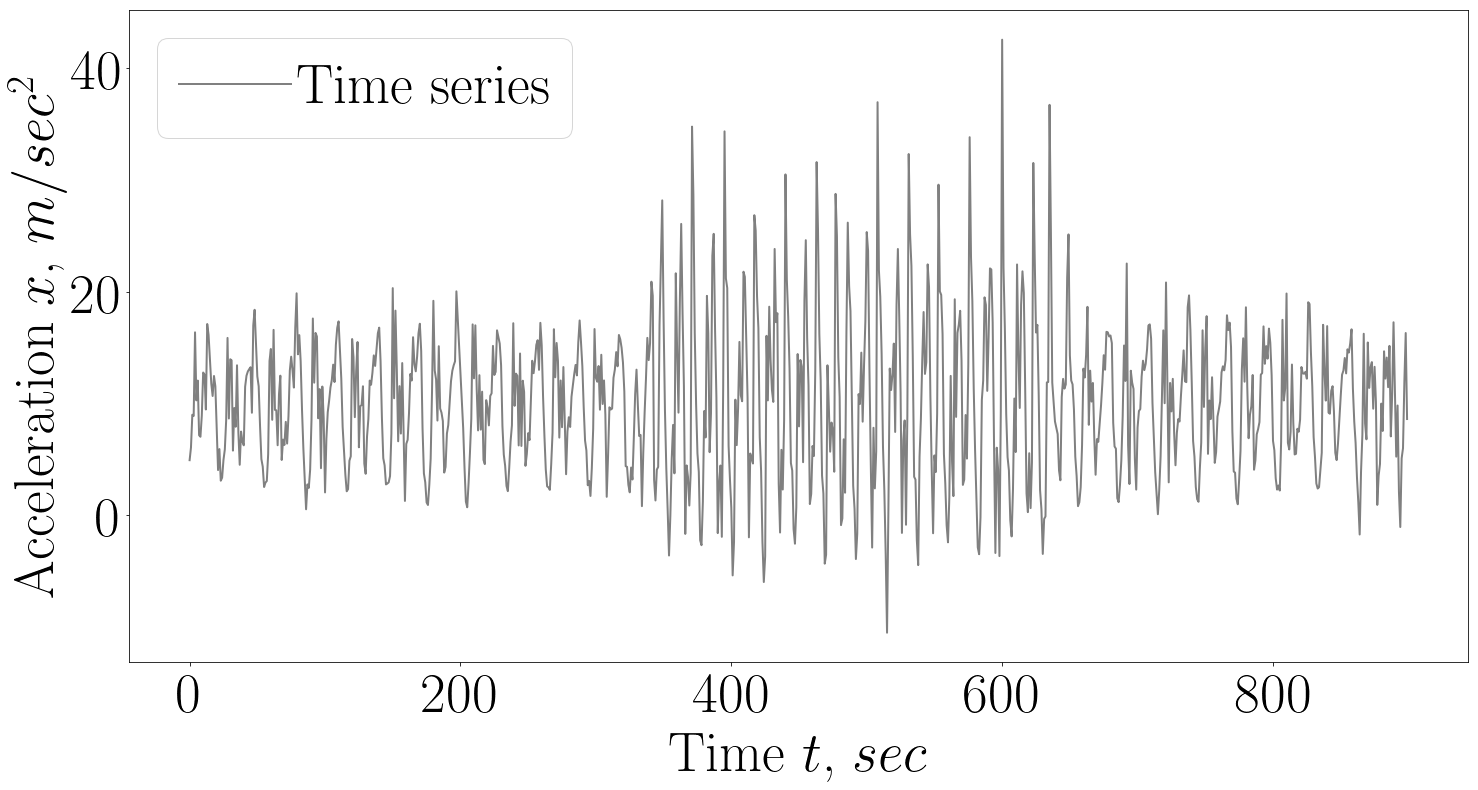
\includegraphics[width=0.5\textwidth]{results/real_1_series}}
\subfloat[]
{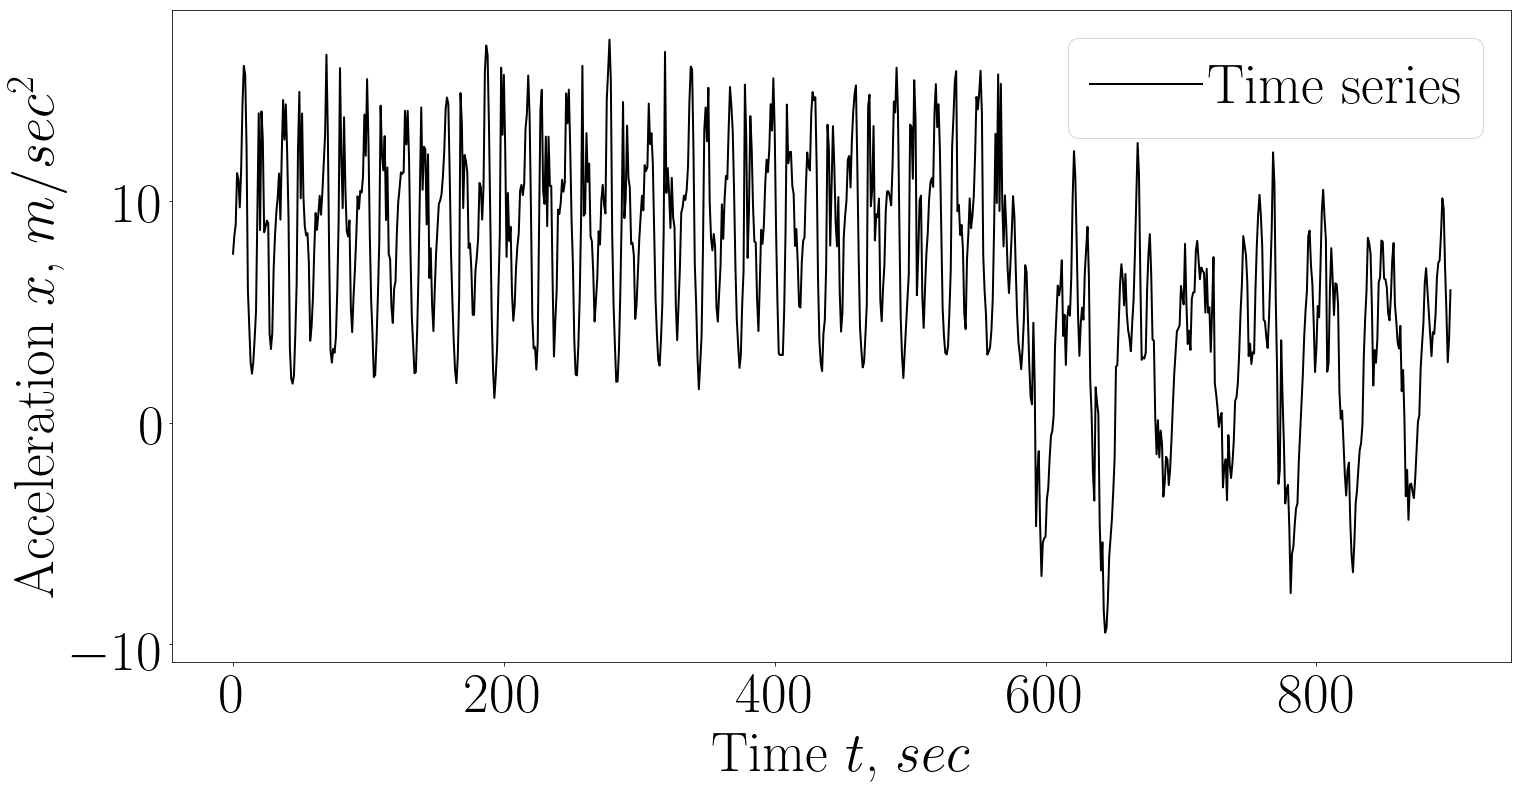
\includegraphics[width=0.5\textwidth]{results/real_2_series}}\\
\caption{Пример синтетически построенных временных рядов: a) для временного ряда Physical~Motion~1; b) для временного ряда Physical~Motion~2}
\label{fig_real_series}
\end{figure}

\begin{figure}[h!t]\center
\subfloat[]
{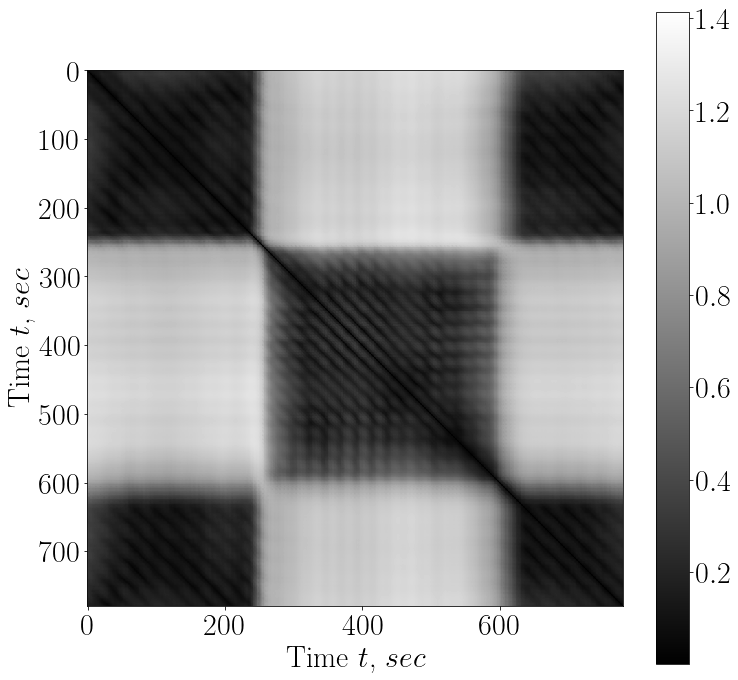
\includegraphics[width=0.5\textwidth]{results/real_1_full}}
\subfloat[]
{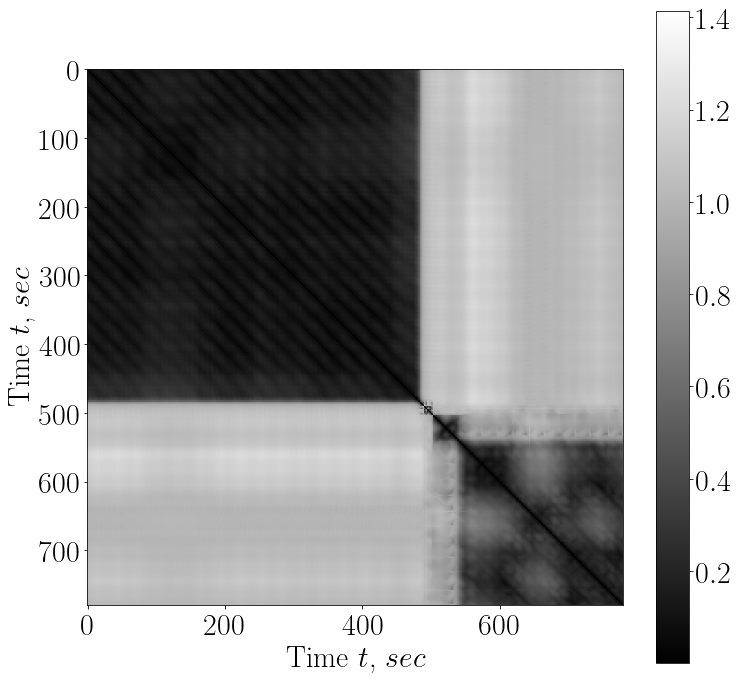
\includegraphics[width=0.5\textwidth]{results/real_2_full}}\\
\caption{Матрица попарных расстояний~$\textbf{M}$ между точками временного ряда: a) для временного ряда Physical~Motion~1; b) для временного ряда Physical~Motion~2}
\label{fig_real_distance}
\end{figure}

\begin{figure}[h!t]\center
\subfloat[]
{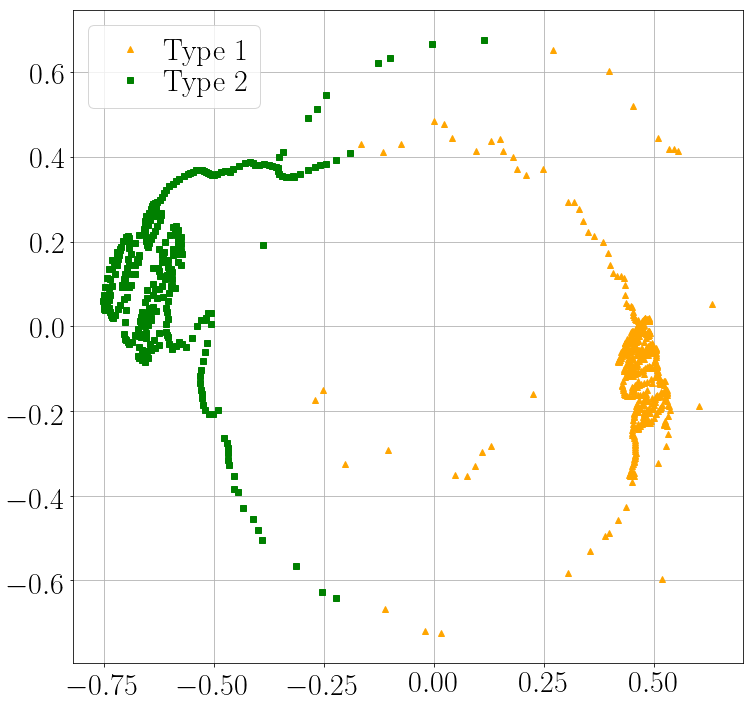
\includegraphics[width=0.5\textwidth]{results/real_1_2D_vector}}
\subfloat[]
{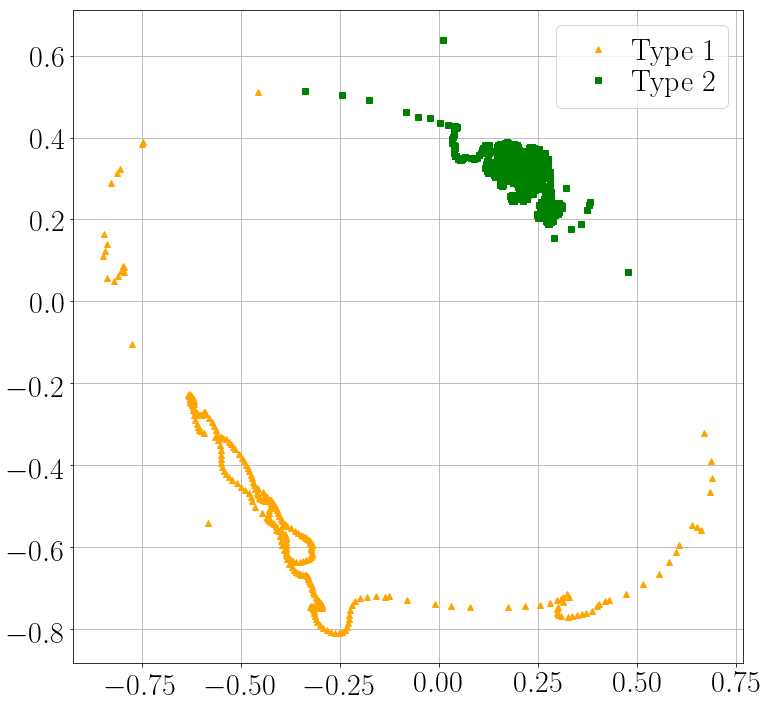
\includegraphics[width=0.5\textwidth]{results/real_2_2D_vector}}\\
\caption{Проекция точек временного на плоскость при помощи матрицы попарных расстояний~$\textbf{M}$: a) для временного ряда Physical~Motion~1; b) для временного ряда Physical~Motion~2}
\label{fig_real_2D}
\end{figure}

\begin{figure}[h!t]\center
\subfloat[]
{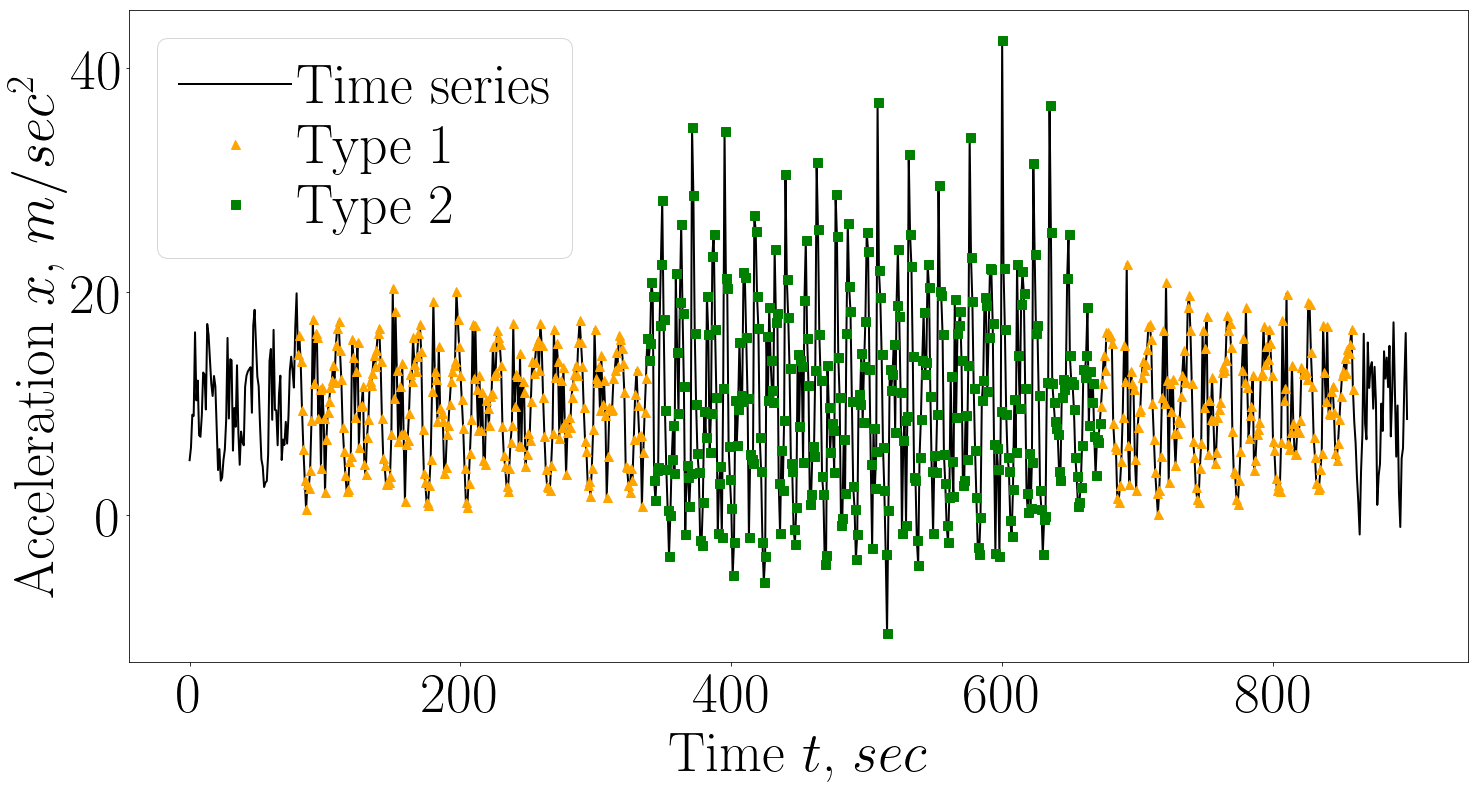
\includegraphics[width=0.5\textwidth]{results/real_1_claster_vector}}
\subfloat[]
{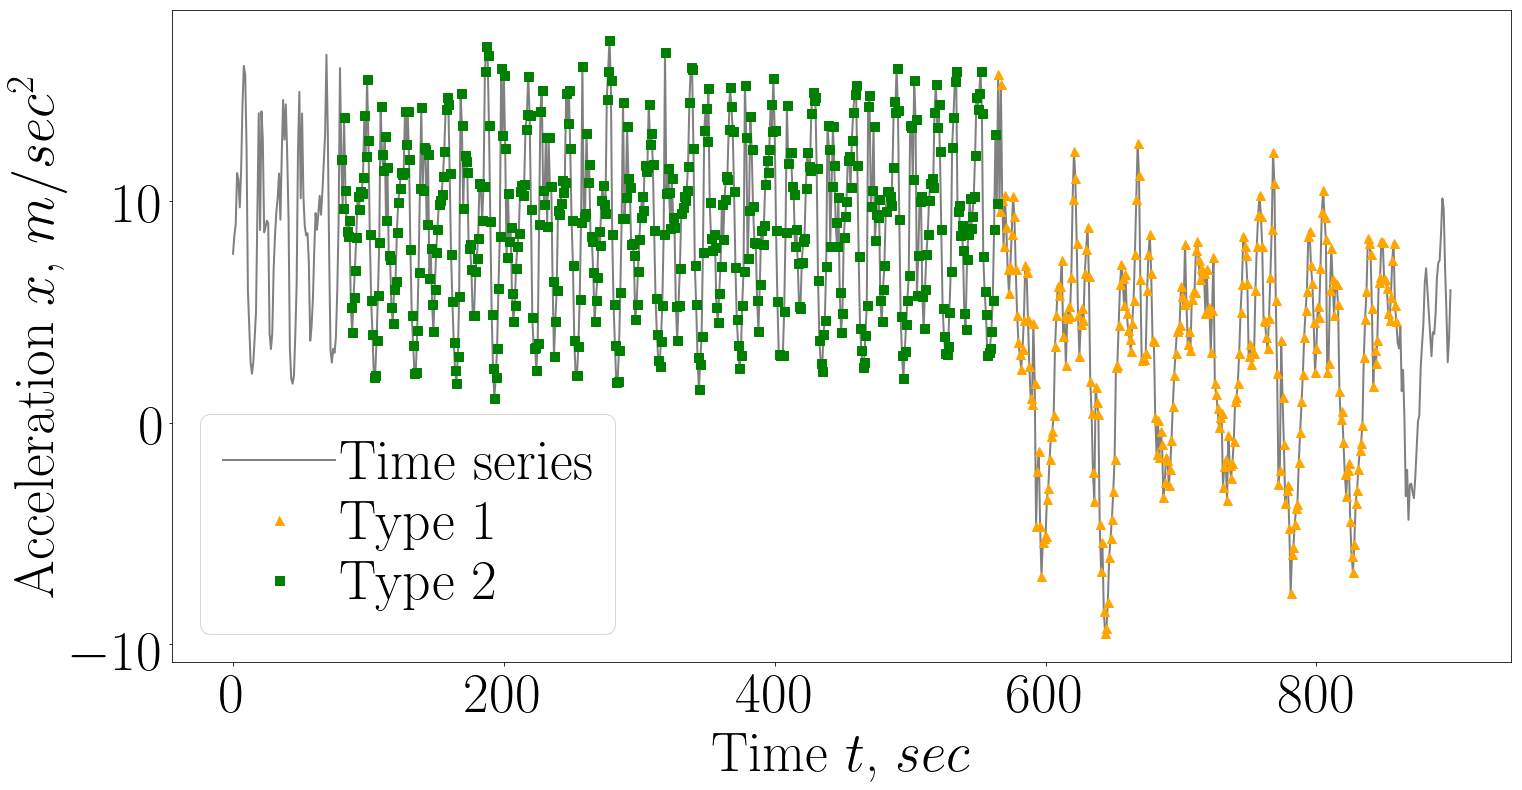
\includegraphics[width=0.5\textwidth]{results/real_2_claster_vector}}\\
\caption{Кластеризация точек временного ряда: 
a) для временного ряда Physical~Motion~1; b) для временного ряда Physical~Motion~2}
\label{fig_real_claster}
\end{figure}

\paragraph{Реальные данные.}

На рис.~\ref{fig_real_series} приведен пример реальных временных рядов полученных при помощи взятия одной из координат мобильного акселерометра. 

Рис.~\ref{fig_real_distance} иллюстрирует матрицы попарных расстояний~$\textbf{M}$ между всеми парами точек~$t$ временного ряда, которые построены при помощи~(\ref{eq:cl:9}). 
Используя матрицу попарных расстояний и метод Multidimensional Scaling~\cite{Borg2005} визуализируем точки временного ряда на плоскости. 
На рис.~\ref{fig_real_2D} показана визуализация точек на плоскости и выполнена их кластеризация при помощи метода иерархической кластеризации. 
Иллюстрация кластеров точек временного ряда продемонстрирована на рис.~\ref{fig_real_claster}.

\subsection{Сегментация временный рядов}
Сегментация временных рядов проводится на синтетических и реальных данных. Для данного эксперимента в качестве синтетического ряда рассматривается ряд построенный из двух синусов с произвольной частотой и амплитудой. Описание временных рядов, которые используются в данном эксперименте представлены в таблице~\ref{table:3}.

Сегментация проводится при помощи метода, который представлен в работе~\cite{motrenko2015}. Данный метод применяется для каждого действия внутри временного ряда по отдельности.


\begin{table}[h!t]
\begin{center}
\caption{Описание временных рядов в эксперименте сегментации временных рядов}
\label{table:3}
\begin{tabular}{|c|c|c|c|}
\hline
	Ряд,~$\textbf{x}$ &Длина ряда,~$N$& Число сегментов,~$K$&Длина сегмента,~$T$\\
	\hline
	\multicolumn{1}{|l|}{Simple~1}
	& 1000& 2& 100\\
	\hline
	\multicolumn{1}{|l|}{Physical~Motion~2}
	& 900& 2& 40\\
\hline

\end{tabular}
\end{center}
\end{table}

\paragraph{Синтетические данные.} На рис.~\ref{fig_simple_segmentation} показан результат работы сегментации для временного ряда Simple~1. 
Данный алгоритм хорошо выделил начала сегментов. 
Также на рис.~\ref{fig_simple_segmentation} показаны проекции фазовых пространств для обеих кластеров на их первые две главные компоненты.

\begin{figure}[h!t]\center
\subfloat[]
{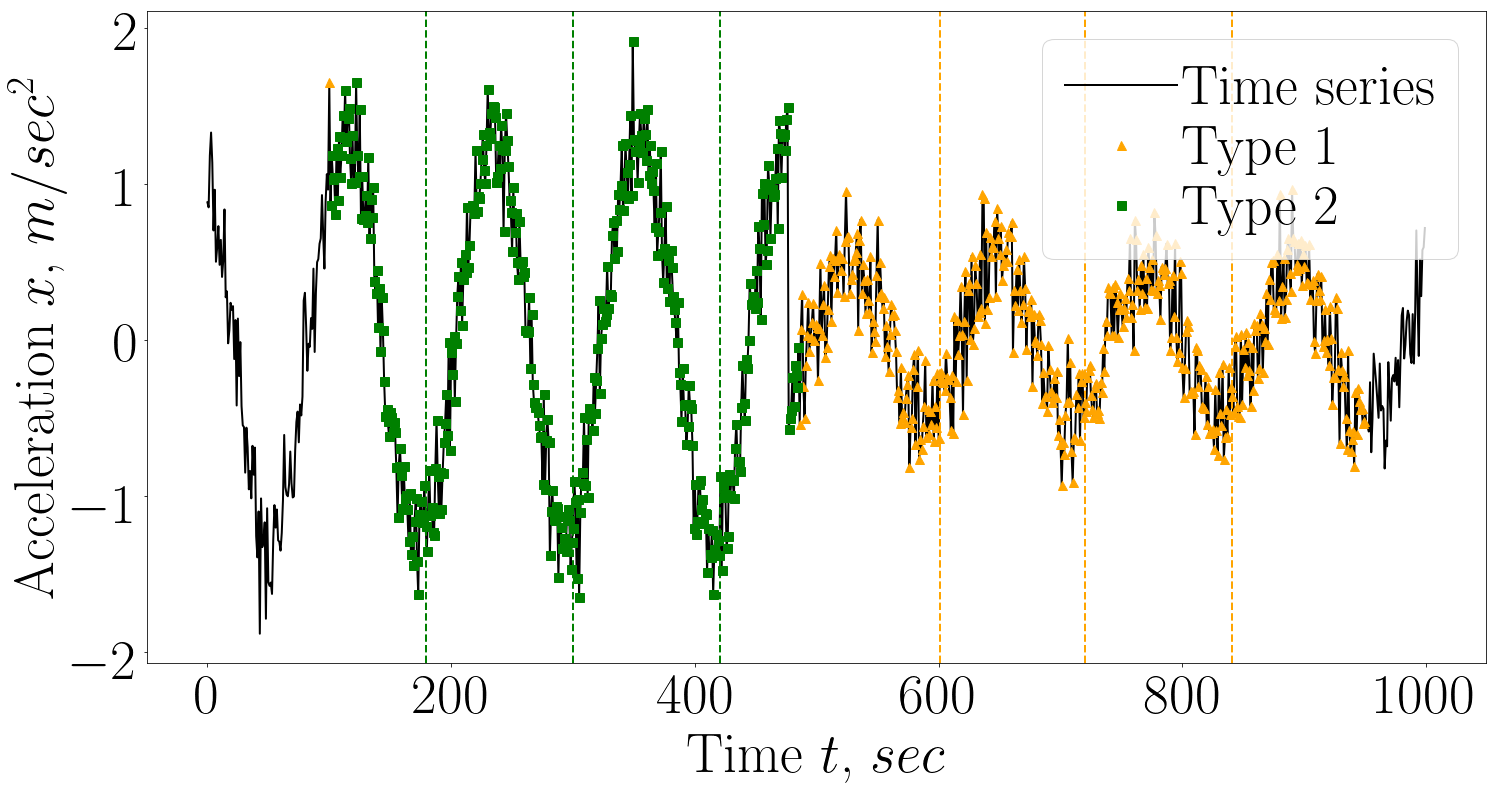
\includegraphics[width=0.5\textwidth]{results/simple_1_segmentation_vector}}
\subfloat[]
{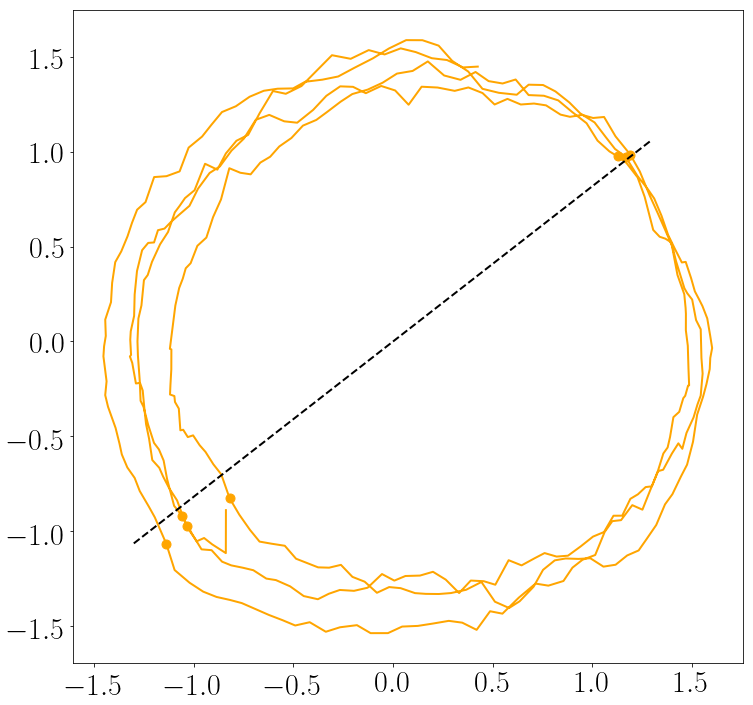
\includegraphics[width=0.25\textwidth]{results/simple_1_phase_space0}}
\subfloat[]
{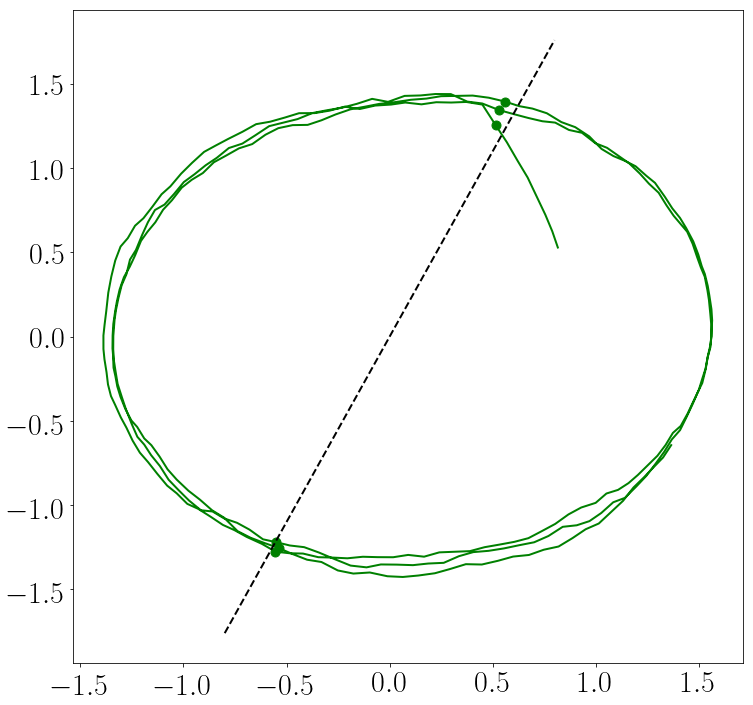
\includegraphics[width=0.25\textwidth]{results/simple_1_phase_space1}}\\
\caption{Сегментация точек временного ряда Simple~1: 
a) сегментация временного ряда; b) проекция фазового пространства на первые две главные компоненты для первого кластера; c) проекция фазового пространства на первые две главные компоненты для второго кластера}
\label{fig_simple_segmentation}
\end{figure}

\paragraph{Реальные данные.} На рис.~\ref{fig_real_segmentation} показан результат работы сегментации для временного ряда Physical~Motion~2. 
Данный алгоритм хорошо выделил начала сегментов для Type~1 и плохо для Type~2. 
Также на рис.~\ref{fig_real_segmentation} показаны проекции фазовых пространств для обеих кластеров на их первые две главные компоненты. 
Видно, что в случае проекции фазового пространства для части ряда, который относится к Type~2 получаем, что фазовая траектория имеет самопересечение внутри одного сегмента, что влечет нахождения ложного начала сегмента.

\begin{figure}[h!t]\center
\subfloat[]
{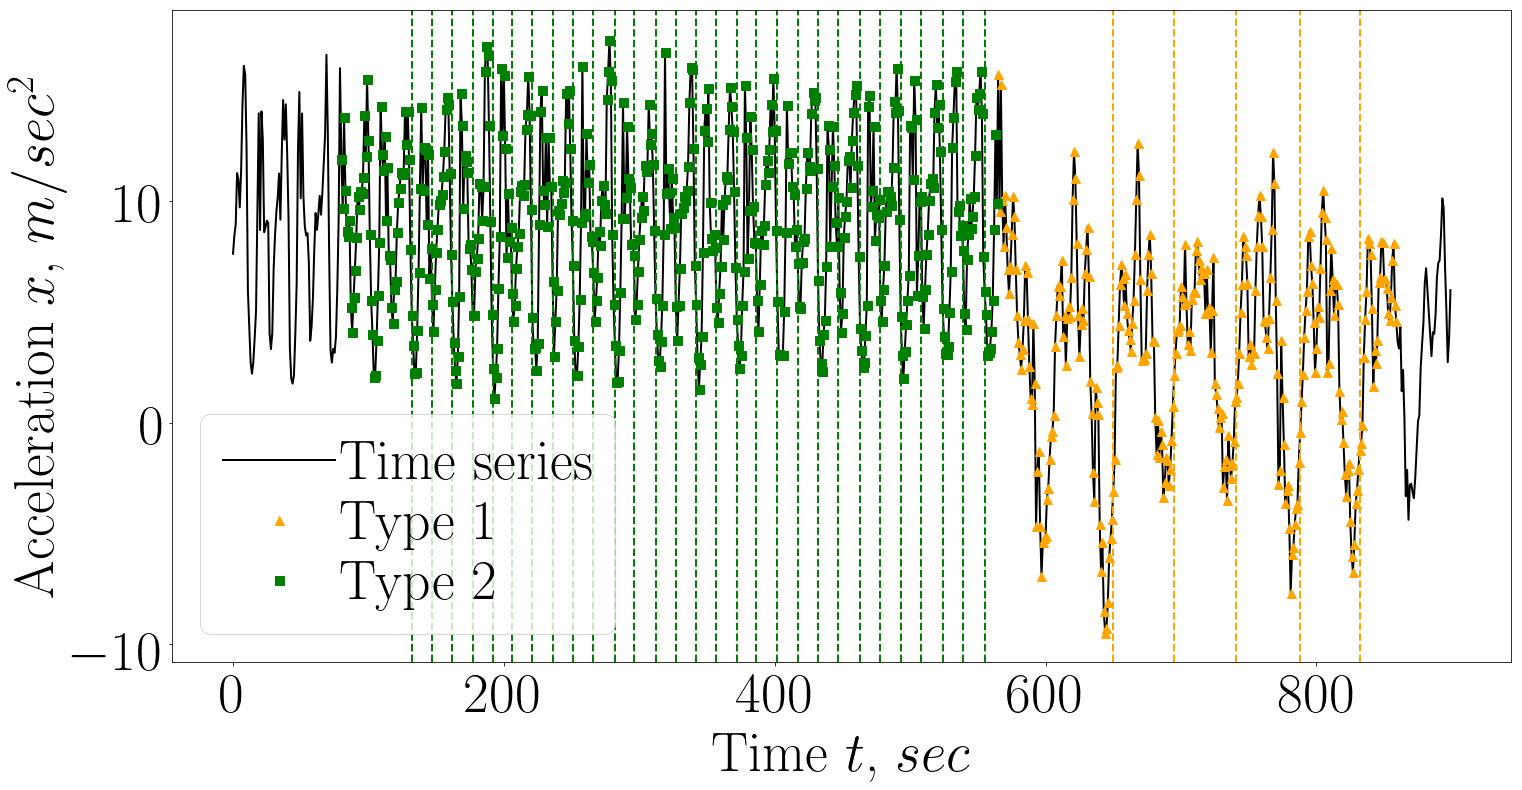
\includegraphics[width=0.5\textwidth]{results/real_2_segmentation_vector}}
\subfloat[]
{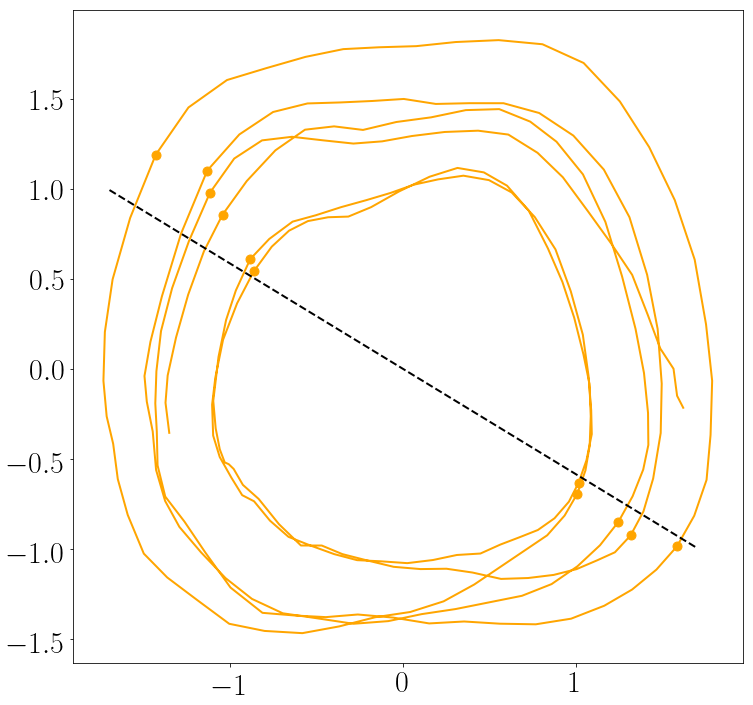
\includegraphics[width=0.25\textwidth]{results/real_2_phase_space0}}
\subfloat[]
{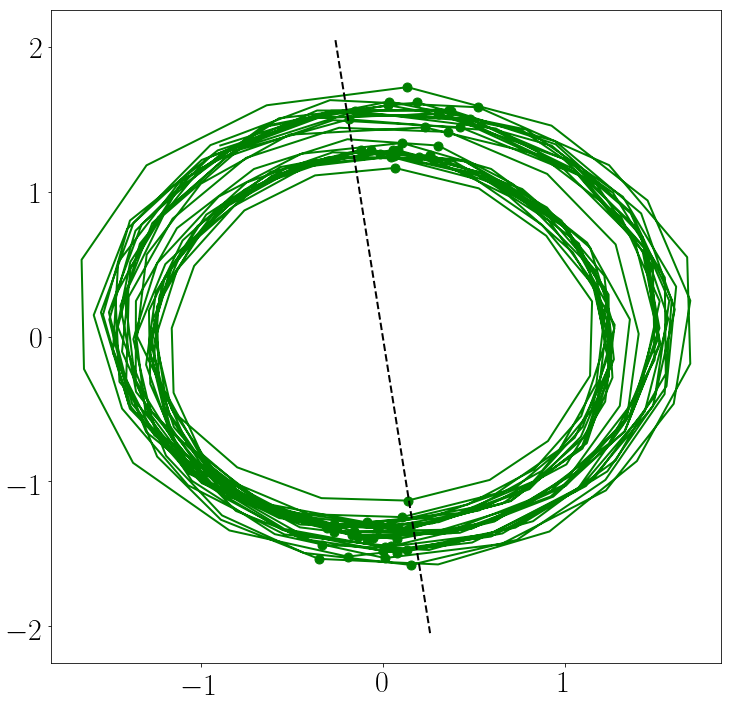
\includegraphics[width=0.25\textwidth]{results/real_2_phase_space1}}\\
\caption{Сегментация точек временного ряда Physical~Motion~2: 
a) сегментация временного ряда; b) проекция фазового пространства на первые две главные компоненты для первого кластера; c) проекция фазового пространства на первые две главные компоненты для второго кластера}
\label{fig_real_segmentation}
\end{figure}

\section{Заключение}
\begin{table}[h!t]
\begin{center}
\caption{Результаты работы алгоритма}
\label{table_2}
\begin{tabular}{|c|c|c|c|c|}
\hline
	Ряд,~$\textbf{x}$ &Длина ряда,~$N$& \# сегментов,~$K$&Длина сегмента,~$T$& Ошибка,~$S$\\
	\hline
	\multicolumn{1}{|l|}{Phys.~Motion~1}
	& 900& 2& 40& 0.06\\
	\hline
	\multicolumn{1}{|l|}{Phys.~Motion~2}
	& 900& 2& 40& 0.03\\
	\hline
	\multicolumn{1}{|l|}{Synthetic~1}
	& 2000& 2& 20& 0.04\\
	\hline
	\multicolumn{1}{|l|}{Synthetic~2}
	& 2000& 3& 20& 0.03\\
\hline

\end{tabular}
\end{center}
\end{table}

В работе рассматривалась задача поиска характерных периодических структур внутри временного ряда. 
Рассматривался метод основаный на локальном снижение размерности фазового пространства. 
Был предложен алгоритм поиска характерных сегментов, который основывается на методе главных компонент для локального снижения размерности. 
Также введена функция расстояния между локальными базисами в каждый момент времени, которые интерпретировались как признаковое описание точки временного ряда.

В ходе эксперимента, на реальных показаниях акселерометра, а также на синтетических данных, было показано, что предложенный метод измерение расстояния между базисами хорошо разделяет точки которые принадлежат различным действиям, что приводит к хорошей кластеризации объектов. 
Результаты работы, показаны в таблице~\ref{table_2}.
Также в эксперименте была проведена полная сегментация временных рядов при помощи метода~\cite{motrenko2015} для каждого кластера по отдельности.

Предложеный метод имеет ряд недостаткров связаных с большим число ограничей на временной ряд. 
Данные ограничения будут ослаблены в последующих работах. Планируется решить задачу нахождения и описания замкнутой фазовой траектории, которая относится к одному квазипериодическому сегменту. 

\begin{comment}
\appendix
\setcounter{theorem}{0}
\section{Теорема (Грабовой 2019)}\label{ProofTheorem1}
\begin{theorem}\label{th:1} 
Пусть задано множество подпространств~$\mathbb{W}$ пространства~$\mathbb{R}^{n}$. Каждое подпространство которого задается базисом~$\mathbf{W}_i\in \mathbf{W}$, тогда функция расстояния~$\rho\left(\textbf{W}_1, \textbf{W}_2\right)$ является метрикой заданой на множестве базисов~$\mathbf{W}$:
\begin{equation}
\begin{aligned}
\rho\left(\textbf{W}_1, \textbf{W}_2\right) = \max\left(\max_{\textbf{e}_2 \in \textbf{W}_2} d_{1}\left(\textbf{e}_2\right), \max_{\textbf{e}_1 \in \textbf{W}_1} d_{2}\left(\textbf{e}_1\right)\right),
\end{aligned}
\end{equation}
где~$\textbf{e}_i$ это базисный вектор из~$\textbf{W}_i$, a~$d_i\left(\textbf{e}\right)$ является расстоянием от вектора~$\textbf{e}$ до пространства заданого базисом~$\textbf{W}_i$.
\end{theorem}
\begin{proof}
Для доказательства данной теоремы, нужно показать, что функция~$\rho$ удовлетворяет трем свойствам метрики.

Функция~$\rho$ удовлетворяет первому свойству метрики:
\begin{equation}
\label{eq:th2:2}
\begin{aligned}
\rho\left(\textbf{W}_1, \textbf{W}_2\right) = 0 \Leftrightarrow \textbf{W}_1 = \textbf{W}_2
\end{aligned}
\end{equation}

Функция~$\rho$ удовлетворяет второму свойству метрики:
\begin{equation}
\label{eq:th2:3}
\begin{aligned}
\rho\left(\textbf{W}_1, \textbf{W}_2\right) = \rho\left(\textbf{W}_2, \textbf{W}_1\right)
\end{aligned}
\end{equation}

Докажем, что функция~$\rho$ удовлетворяет удовлетворяет неравенству треугольника:
\begin{equation}
\label{eq:th2:4}
\begin{aligned}
\rho\left(\textbf{W}_1, \textbf{W}_2\right) \leq \rho\left(\textbf{W}_1, \textbf{W}_3\right) + \rho\left(\textbf{W}_3, \textbf{W}_2\right)
\end{aligned}
\end{equation}

Для доказательства неравенства треугольника докажем неравенства:
\begin{equation}
\label{eq:th2:5}
\begin{aligned}
\max_{\textbf{e}_1 \in \textbf{W}_1}d_{2}\left(\textbf{e}_1\right) \leq 
\max_{\textbf{e}_1\in \textbf{W}_1}d_{3}\left(\textbf{e}_1\right)+
\max_{\textbf{e}_3 \in \textbf{W}_3}d_{2}\left(\textbf{e}_3\right) \\
\max_{\textbf{e}_2 \in \textbf{W}_2}d_{1}\left(\textbf{e}_2\right) \leq 
\max_{\textbf{e}_2\in \textbf{W}_2}d_{3}\left(\textbf{e}_2\right)+
\max_{\textbf{e}_3 \in \textbf{W}_3}d_{1}\left(\textbf{e}_3\right)
\end{aligned}
\end{equation}

Используя Лемму~\ref{lem:1} доказательство неравенства (\ref{eq:th2:5}) сводится к доказательства неравенства:
\begin{equation}
\label{eq:th2:6}
\begin{aligned}
\max_{\substack{\textbf{a} \in \textbf{W}_1 \\ \left|\textbf{a}\right| \leq 1}}d_{2}\left(\textbf{a}\right) \leq 
\max_{\substack{\textbf{a} \in \textbf{W}_1 \\ \left|\textbf{a}\right| \leq 1}}d_{3}\left(\textbf{a}\right)+
\max_{\substack{\textbf{c} \in \textbf{W}_3 \\ \left|\textbf{c}\right| \leq 1}}d_{2}\left(\textbf{c}\right),
\end{aligned}
\end{equation}
где~$\textbf{a}, \textbf{c}$ произвольные элементы из соответствующих подпространств. 

Подставив в выражение~(\ref{eq:th2:6}) выражение для~$h_i\left(\textbf{a}\right)$, получаем следующее неравенство:
\begin{equation}
\label{eq:th2:7}
\begin{aligned}
\max_{\substack{\textbf{a} \in \textbf{W}_1 \\ \left|\textbf{a}\right| \leq 1}} \min_{\substack{\textbf{b} \in \textbf{W}_2 \\ \left|\textbf{b}\right| \leq 1}}||\textbf{a} - \textbf{b}|| \leq 
\max_{\substack{\textbf{a} \in \textbf{W}_1 \\ \left|\textbf{a}\right| \leq 1}} \min_{\substack{\textbf{c} \in \textbf{W}_3 \\ \left|\textbf{b}\right| \leq 1}}||\textbf{a} - \textbf{c}||+
\max_{\substack{\textbf{c} \in \textbf{W}_3 \\ \left|\textbf{c}\right| \leq 1}} \min_{\substack{\textbf{b} \in \textbf{W}_2 \\ \left|\textbf{b}\right| \leq 1}}||\textbf{c} - \textbf{b}||.
\end{aligned}
\end{equation}

Неравенство~(\ref{eq:th2:7}) следует из Леммы~\ref{lem:2}. Из выполнения неравенства~(\ref{eq:th2:7}) следует выполнение неравенств~(\ref{eq:th2:5}).
Докажем неравенство треугольника~(\ref{eq:th2:4}) используя неравенства~(\ref{eq:th2:5}). Для удобства введем следующие обозначения:
\begin{equation}
\label{eq:th2:8}
\begin{aligned}
\max_{\textbf{e}_i \in \textbf{W}_i} d_j\left(\textbf{e}_i\right) = d_{i}^{j}.
\end{aligned}
\end{equation}

Из истинности неравенства~(\ref{eq:th2:7}) в обозначениях~(\ref{eq:th2:8}) следует истинность следующих неравенств:
 
\begin{equation}
\label{eq:th2:9}
\begin{aligned}
\quad d_{1}^{2} \leq d_{1}^{3} + d_{3}^{2} \leq \max\left(d_{1}^{3}, d_{3}^{1}\right) + \max\left(d_{3}^{2}, d_{2}^{3}\right)\\
\quad h_{2}^{1} \leq d_{2}^{3} + d_{3}^{1} \leq \max\left(d_{2}^{3}, d_{3}^{2}\right) + \max\left(d_{3}^{1}, h_{1}^{3}\right)\\
\end{aligned}
\end{equation}

Из уравнения~(\ref{eq:th2:9}) следует выполнение неравенства:
\begin{equation}
\label{eq:th2:10}
\begin{aligned}
\max\left(d_{1}^{2}, d_{2}^{1}\right) \leq  \max\left(d_{1}^{3}, d_{3}^{1}\right) + \max\left(d_{3}^{2}, d_{2}^{3}\right)\\
\end{aligned}
\end{equation}

Доказательство неравенства~(\ref{eq:th2:10}) указывает на выполнение неравенства треугольника для функции~$\rho$, что завершает доказательство того, что~$\rho$ является метрикой.

\end{proof}


\begin{lemma} \label{lem:1} 
Пусть заданы два подпространства~$\mathbb{X}, \mathbb{Y} \subset \mathbb{R}^{n}$, которые задаются базисами~$\textbf{W}_1$ и~$\textbf{W}_2$, тогда справедливо следующее условие:

\begin{equation}
\label{eq:l1:1}
\begin{aligned}
\max_{\textbf{a} \in \mathbb{X}:~\left|\textbf{a}\right|\leq 1}d_2\left(\textbf{a}\right) = \max_{\textbf{a} \in \mathbb{X}:~\left|\textbf{a}\right|= 1}d_2\left(\textbf{a}\right)
\end{aligned}
\end{equation}
где~$d_i\left(\textbf{a}\right)$ является расстоянием от вектора~$\textbf{a}$ до пространства заданого базисом~$\textbf{W}_i$.
\end{lemma}

\begin{proof}
\begin{equation}
\label{eq:l1:2}
\begin{aligned}
\max_{\textbf{a} \in \mathbb{X}:~\left|\textbf{a}\right|\leq 1}d_2\left(\textbf{a}\right) = \max_{\textbf{a} \in \mathbb{X}:~\left|\textbf{a}\right|\leq 1}\left|\textbf{a}-\sum_{i}\langle \textbf{e}^i_2, \textbf{a} \rangle\textbf{e}^i_2 \right| = \\ 
=\max_{\{\alpha_j\}_{j}:~\sum\alpha_j^2\leq 1}\left|\sum_{j}\alpha_j\textbf{e}^{j}_1-\sum_{i}\langle \textbf{e}^i_2, \sum_{j}\alpha_j\textbf{e}^{j}_1 \rangle\textbf{e}^i_2 \right| =\\
= \max_{\{\alpha_j\}_{j}:~\sum\alpha_j^2\leq 1}\left|\sum_{j}\alpha_j\left(\textbf{e}_3^j - \sum_{i}\langle\textbf{e}_3^j,\textbf{e}_2^i\rangle\textbf{e}_2^i\right)\right|,
\end{aligned}
\end{equation}
где в выражении~(\ref{eq:l1:2}) максимум очевидно достигается на~$j$-ом базисном векторе для которого выражение в скобках является максимальным.
\end{proof}




\begin{lemma} \label{lem:2} 
Пусть заданы подпространства~$\mathbb{X}, \mathbb{Y}, \mathbb{Z} \subset \mathbb{R}^{n}$, которые задаются базисами~$\textbf{W}_1, \textbf{W}_2, \textbf{W}_3$ соответственно, тогда справедливо следующее условие:

\begin{equation}
\label{eq:l2:1}
\begin{aligned}
\max_{\substack{\textbf{x} \in \mathbb{X} \\ \left|\textbf{x}\right|\leq 1}}\min_{\substack{\textbf{y} \in \mathbb{Y} \\ \left|\textbf{y}\right|\leq 1}}||\textbf{x}-\textbf{y}||\leq 
\max_{\substack{\textbf{x} \in \mathbb{X} \\ \left|\textbf{x}\right|\leq 1}}\min_{\substack{\textbf{z} \in \mathbb{Z} \\ \left|\textbf{z}\right|\leq 1}}||\textbf{x}-\textbf{z}|| + 
\max_{\substack{\textbf{z} \in \mathbb{Z} \\ \left|\textbf{z}\right|\leq 1}}\min_{\substack{\textbf{y} \in \mathbb{Y} \\ \left|\textbf{y}\right|\leq 1}}||\textbf{z}-\textbf{y}||.
\end{aligned}
\end{equation}
\end{lemma}

\begin{proof} 
\begin{equation}
\label{eq:l2:2}
\begin{aligned}
\max_{\substack{\textbf{x} \in \mathbb{X} \\ \left|\textbf{x}\right|\leq 1}}\min_{\substack{\textbf{y} \in \mathbb{Y} \\ \left|\textbf{y}\right|\leq 1}}||\textbf{x}-\textbf{y}||\leq
\max_{\substack{\textbf{x} \in \mathbb{X} \\ \left|\textbf{x}\right|\leq 1}}\min_{\substack{\textbf{y} \in \mathbb{Y} \\ \left|\textbf{y}\right|\leq 1}}\left(||\textbf{x}-\textbf{z}|| + ||\textbf{z} - \textbf{y}||\right) = \\
\max_{\substack{\textbf{x} \in \mathbb{X} \\ \left|\textbf{x}\right|\leq 1}}||\textbf{x}-\textbf{z}|| + \min_{\substack{\textbf{y} \in \mathbb{Y} \\ \left|\textbf{y}\right|\leq 1}}||\textbf{z} - \textbf{y}|| = \max_{\substack{\textbf{x} \in \mathbb{X} \\ \left|\textbf{x}\right|\leq 1}}\min_{\substack{\textbf{z} \in \mathbb{Z} \\ \left|\textbf{z}\right|\leq 1}}||\textbf{x}-\textbf{z}|| + \min_{\substack{\textbf{y} \in \mathbb{Y} \\ \left|\textbf{y}\right|\leq 1}}||\textbf{z} - \textbf{y}|| \leq \\
\leq \max_{\substack{\textbf{x} \in \mathbb{X} \\ \left|\textbf{x}\right|\leq 1}}\min_{\substack{\textbf{z} \in \mathbb{Z} \\ \left|\textbf{z}\right|\leq 1}}||\textbf{x}-\textbf{z}|| + 
\max_{\substack{\textbf{z} \in \mathbb{Z} \\ \left|\textbf{z}\right|\leq 1}}\min_{\substack{\textbf{y} \in \mathbb{Y} \\ \left|\textbf{y}\right|\leq 1}}||\textbf{z}-\textbf{y}||.
\end{aligned}
\end{equation}
\end{proof}

\end{comment}

\begin{thebibliography}{99}
	\bibitem{kwapisz2010}
	\textit{J. R. Kwapisz, G. M. Weiss, S. A. Moore} Activity Recognition using Cell Phone Accelerometers~// Proceedings of the Fourth International Workshop on Knowledge Discovery from Sensor Data, 2010. Vol. 12. P. 74--82.
	
	\bibitem{wang2014}
	\textit{W. Wang, H. Liu, L. Yu, F. Sun} Activity Recognition using Cell Phone Accelerometers~// Joint Conference on Neural Networks, 2014. P. 1185--1190.
	
	\bibitem{Ignatov2015}
	\textit{A. D. Ignatov, V. V. Strijov} Human activity recognition using quasiperiodic time series collected from a single tri-axial accelerometer.~// Multimedial Tools and Applications, 2015.
	
	\bibitem{Olivares2012}
	\textit{A. Olivares, J. Ramirez, J. M. Gorris, G. Olivares, M. Damas} Detection of (in)activity periods in human body motion using inertial sensors: A comparative study.~// Sensors, 12(5):5791–5814, 2012.
	
	\bibitem{cinar2018}
	\textit{Y. G. Cinar and H. Mirisaee} Period-aware content attention RNNs for time series forecasting with missing values~// Neurocomputing, 2018. Vol. 312. P. 177--186.
	
	\bibitem{motrenko2015}
	\textit{A. P. Motrenko, V. V. Strijov} Extracting fundamental periods to segment biomedical signals~// Journal of Biomedical and Health Informatics, 2015,~20(6). P.~1466~-~1476.
	
	\bibitem{lukashin2003}
	\textit{Y. P. Lukashin} Adaptive methods for short-term forecasting~// Finansy and Statistik, 2003.
	
	\bibitem{Ivkin2015}
	\textit{И. П. Ивкин,  М. П. Кузнецов} Алгоритм классификации временных рядов акселерометра по комбинированному признаковому описанию.~// Машинное обучение и анализ данных, 2015.
	
	\bibitem{Katrutsa2015}
	\textit{V. V. Strijov, A. M. Katrutsa} Stresstes procedures for features selection algorithms.~// Schemometrics and Intelligent Laboratory System, 2015.
	
	\bibitem{Borg2005}
	\textit{I. Borg, P. J. F. Groenen} Modern Multidimensional Scaling. --- New York: Springer, 2005. 540 p.
	
	%\bibitem{Kanungo2000}
	%\textit{T. Kanungo, D. M. Mount et al} An Efficient k-Means Clustering Algorithm: Analysis and Implementation. 2000.
	
	\bibitem{Shiglavsi1997}
	\textit{Д. Л. Данилова, А. А. Жигловский} Главные компоненты временных рядов: метод "Гусеница".~---~Санкт-Петербурскиий университет, 1997.
	

	
\end{thebibliography}

\end{document}

